\documentclass[sigconf,nonacm]{acmart}

\usepackage{amsmath}
\usepackage{amsfonts}
\let\Bbbk\undefined
\usepackage{amssymb}
\usepackage{booktabs}
\usepackage{multirow}
\usepackage{graphicx}
\usepackage{algorithm}
\usepackage{algorithmic}
\graphicspath{{../results/}{./}}

\settopmatter{printacmref=false}
\setcopyright{none}
\renewcommand\footnotetextcopyrightpermission[1]{}
\pagestyle{plain}

% Math shortcuts
\newcommand{\eps}{\varepsilon}
\newcommand{\E}{\mathbb{E}}
\newcommand{\Prob}{\mathbb{P}}
\newcommand{\Lap}{\mathrm{Lap}}
\DeclareMathOperator{\Var}{Var}
\newtheorem{prop}{Proposition}
\newtheorem{defn}{Definition}

\begin{document}

\title{Forecasting Privacy-Budget Consumption in Repeated DP-SQL Workloads}
\author{Can \"Ozta\c{s}}
\affiliation{%
 \institution{Hacettepe University}
 \city{Ankara}
 \country{Turkey}
}
\email{canoztas06@gmail.com}

\author{Engin Demir}
\affiliation{%
 \institution{Hacettepe University}
 \city{Ankara}
 \country{Turkey}
}
\email{engindemir@hacettepe.edu.tr}

\begin{abstract}
Differentially private (DP) SQL systems add calibrated noise to each aggregate query and charge it against a finite privacy budget; once the budget is exhausted, no further query can be answered. Existing systems account for each query in isolation, although workloads repeat heavily and an exact repeat is free by post-processing. A data custodian therefore cannot tell in advance whether a workload will fit its budget. We present a closed-form model that forecasts a workload's budget consumption before any query executes, from public repetition structure alone: the distribution over distinct queries, the workload length, and the budget. The model yields the expected spend, a hard completion guarantee under a safe per-query budget, and a per-release accuracy verdict. Being mechanism-agnostic, it extends to Markovian and regime-switching arrivals and transfers unchanged to multi-table joins. The forecast is the accounting core of a DP-SQL middleware we implement over DuckDB and PostgreSQL: it sizes the budget allocator, gates temporal re-releases, and prices equivalence-aware caching. Across a $4{,}155$-trial campaign the forecast matches observed consumption within $3\%$ in $21$ of $24$ configurations, and on $30$ workloads derived from real Amazon Redshift traces, forecasting from the first half of each workload reduces the budget-prediction error by $45\%$.
\end{abstract}

\maketitle

%% ============================================================
\section{Introduction and Motivation}
\label{sec:intro}

Aggregate statistics computed over sensitive data leak information about the individuals they summarize. A pair of COUNT queries that differ by one predicate reveals an individual's attribute by differencing; repeated over a dataset, such queries reconstruct it~\cite{dinur2003revealing}. Differential privacy (DP)~\cite{dwork2006calibrating,dwork2014algorithmic} is the standard defense: perturb each answer with noise calibrated to the query's sensitivity and a per-query budget $\eps_q$, and bound the cumulative privacy loss by composition. The budget is a hard, non-renewable resource: once the total $\sum\eps_q$ reaches a cap $B$, no further query can be answered without breaking the guarantee. A data custodian therefore needs to understand, and ideally predict, \emph{how fast a workload spends its budget}.

The need for such a prediction is best illustrated with a concrete scenario. Consider an analytics team that publishes a privacy-protected dashboard: a fixed set of tiles (counts, sums, group-by breakdowns) refreshed on a schedule, plus occasional ad-hoc drill-downs. The custodian sets a monthly budget $B$ and a per-query $\eps_q$. Two failures follow from treating queries in isolation. If $\eps_q$ is set to meet an accuracy target, naive composition exhausts $B$ after only $B/\eps_q$ releases, and the dashboard can no longer be refreshed for the remainder of the month. If $\eps_q$ is set small enough to survive the month, every tile is needlessly noisy. The custodian cannot tell in advance which will happen, because no model relates the \emph{shape} of the workload (how much it repeats) to the budget it will spend. That repetition is precisely the structure our model exploits: the same dashboard tiles recur, so the budget is governed by the handful of \emph{distinct} templates rather than by the hundreds of refreshes.

Existing systems do not exploit this repetition. Most DP-SQL systems (PINQ~\cite{mcsherry2009privacy}, Chorus~\cite{johnson2020chorus}, DOP-SQL~\cite{yu2024dopsql}) charge every query a fresh $\eps_q$ and account for it in isolation (PrivateSQL~\cite{kotsogiannis2019privatesql} instead amortizes a one-time synopsis budget---Section~\ref{sec:related}---but still fixes that budget up front rather than forecasting it). Yet analytical workloads are highly repetitive. A monitoring dashboard re-issues the \emph{exact same} key performance indicator (KPI) tile on a schedule (a canonicalized exact-query repeat, served free), whereas a drill-down reuses a structural template with \emph{different} literals (a distinct exact query that is charged afresh). Only exact repeats save budget; the savings come from how often a dashboard re-issues identical queries. Under exact-repeat caching, a repeated answer is free: re-using an already-released noisy value adds no privacy cost, since any function of a DP output is itself DP (DP's \emph{post-processing} property). Consequently, the budget a workload of length $k$ consumes is governed not by $k$ but by its number of \emph{distinct} queries $u_k$ (Figure~\ref{fig:concept}). The central question of this project is whether $u_k$, and hence the budget, can be \emph{predicted from the workload's repetition structure} in closed form, before the workload runs. Exact-repeat caching itself is a known mechanism and we claim no novelty for it; our contribution is \emph{forecasting} its budget impact \emph{before} execution.

\begin{figure}[t]
\centering
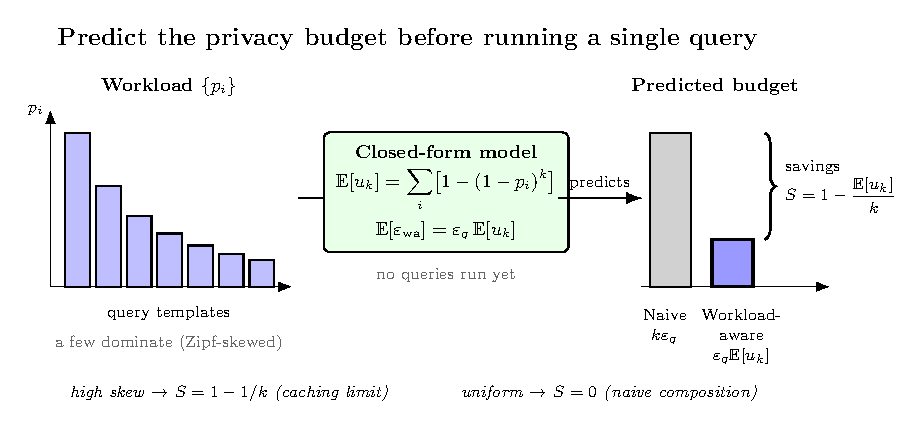
\includegraphics[width=0.95\columnwidth]{fig_concept}
\caption{Naive composition charges every one of $k$ queries; workload-aware accounting charges only the $u_k$ distinct queries (a template together \emph{with} its WHERE literals), since exact repeats are served from cache by post-processing. The model predicts $\E[u_k]$, and hence the budget, before execution.}
\label{fig:concept}
\end{figure}

\subsubsection*{Contributions}
This work makes three contributions.
\begin{enumerate}
 \item \textbf{A before-execution budget forecast for repeated DP-SQL workloads}, to our knowledge the first that is \emph{closed-form} and reads only public structure---the distinct-query distribution $\{p_i\}$, the workload length $k$, and the budget $B$---never touching the data. Before any query executes, the forecast tells a data custodian how much of the budget the workload will consume and whether the workload fits within it. It delivers three outputs of differing strength. The first is the \emph{expected} spend $\eps_q\E[u_k]$, an average-case estimate. The second, under the safe sizing $\eps_q{=}B/m$, is a \emph{hard} completion guarantee, since $u_k\le m$ in the static regime. The third is a \emph{per-release} $(\alpha,\beta)$-accuracy verdict: each release \emph{individually} has error at most $\alpha$ with probability $\ge1-\beta$; this is not a joint guarantee that every release succeeds simultaneously (Section~\ref{sec:method}). No existing DP-SQL system natively exposes such a workload-level forecast (Section~\ref{sec:related}). Five propositions establish this core model (expected distinct count, savings, the Zipf-skew case, a concentration bound, and per-query utility), with two limits recovering the folklore $1-1/k$ caching rule and standard per-query accounting; six further propositions extend it to temporal re-release, Markovian and regime-switching arrivals, and joins (eleven in total).
 \item \textbf{A measured forecasting improvement on production-derived traces.} On $30$ Redbench workloads (synthesized from real Amazon Redshift query traces), forecasting the full distinct-query count from only the \emph{first half} of each workload---via an unseen-species correction---cuts the normalized budget-prediction error, measured as mean absolute error (MAE), by $45\%$ ($0.22\!\to\!0.12$) relative to the plug-in estimate (Section~\ref{sec:redbench}).
 \item \textbf{A workload-aware middleware architecture and a validation campaign.} The forecast is not an add-on to an existing cache but the accounting core of the middleware: the same closed form sizes the budget allocator (the safe $\eps_q{=}B/m$ and the predictive $\eps_q{=}B/\hat U$), gates temporal re-releases (Proposition~\ref{prop:barr}), and prices equivalence classes rather than query strings. We instantiate this architecture over DuckDB and PostgreSQL (equivalence-aware caching, a temporal staleness/update extension, and top-$k$ as DP post-processing) and validate the forecast on a $4{,}155$-trial campaign---within $<3\%$ in $21/24$ cells, invariant to data scale and to $\eps_q$, and exact on a constructed mixed workload---with two leakage experiments confirming the per-query calibration. For reproducibility, the complete implementation, the $233$-test suite, and a generator script for every reported table and figure are publicly available with fixed random seeds, so that all results can be regenerated from a fresh checkout (Section~\ref{sec:discussion}).
\end{enumerate}
We do \emph{not} claim to outperform deployed DP systems. The $100\times$ saving over naive composition is a secondary demonstration of the mechanism, the $1.8\times$ advantage over a learned bandit is an allocator ablation, and the savings we achieve against reactive DP caches (Turbo, CacheDP) are \emph{on par} with theirs. The contribution is the before-execution forecast they do not natively expose (Section~\ref{sec:results}). The headline grid is a self-consistency check (Section~\ref{sec:discussion}); the predictive allocator and the learned-allocator comparison are presented in Appendix~\ref{app:allocator}, and the semantic-caching negative result in Appendix~\ref{app:semantic}.

%% ============================================================
\section{Related Work}
\label{sec:related}

Prior work relevant to our forecast falls into four lines: DP-SQL systems, workload-aware DP and caching, multi-query accounting and online budget allocation, and distinct-count estimation. We review each in turn.

The first line consists of DP-SQL systems. PINQ~\cite{mcsherry2009privacy} introduced composable DP query operators; Chorus~\cite{johnson2020chorus} rewrites SQL to enforce DP; DOP-SQL~\cite{yu2024dopsql} tunes per-query mechanisms. Each exposes a \emph{fixed} per-query $\eps_q$ chosen up front and accounts for queries in isolation. PrivateSQL~\cite{kotsogiannis2019privatesql} is different in kind: it spends a one-time budget building DP synopses (private materialized views) over a \emph{representative} workload, then answers subsequent queries from those synopses with \emph{no} additional privacy loss. This is amortization across a declared query set rather than per-query accounting. None of them \emph{forecasts} a repeated workload's aggregate consumption from its repetition structure. PrivateSQL, for instance, fixes its synopsis budget up front from a representative set but emits no closed-form, before-execution prediction of the savings ratio $S(k)$ (formalized in Section~\ref{sec:method}) for an arbitrary repeated stream.

A second line makes the DP mechanism workload-aware or adds a cache. The matrix mechanism~\cite{li2015matrix} optimizes noise for a \emph{known} batch of linear queries, and Dong, Sun, and Yi~\cite{dong2023better} beat worst-case composition by exploiting relational structure. DP caches make repeated work cheaper at runtime: Turbo~\cite{kostopoulou2023turbo} conserves $1.7$--$15.9\times$ budget by generalizing across overlapping linear queries, and CacheDP~\cite{mazmudar2023cachedp} answers a workload at lower budget under an accuracy contract. Two \emph{proactive} systems are closest to our setting. Pioneer~\cite{peng2013pioneer} reused past noisy results to answer a new query more cheaply, sometimes for free, but by its authors' own statement it optimizes only the \emph{current} query and leaves future-workload effects open; LAPRAS~\cite{mundra2026lapras} precomputes an offline batch mechanism on a \emph{predicted} query set before the stream arrives and serves it at no extra cost---but it needs a concrete predicted set and \emph{touches the sensitive data} ahead of time, whereas we forecast in closed form from \emph{public} repetition structure $(\{p_i\},k,B)$ alone, without touching the data. All of these systems deliver the \emph{savings} our model prices, but they do so reactively (Turbo, CacheDP, Pioneer) or by precomputing on the data (LAPRAS), and none provides a closed-form structural forecast. Our exact-repeat caching is a simple special case, and the mechanism itself carries no novelty claim (Section~\ref{sec:results}).

A third line addresses multi-query accounting and online budget allocation. Tight composition---the moments accountant~\cite{abadi2016deep}, R\'enyi DP~\cite{mironov2017renyi}, and zero-concentrated DP (zCDP)~\cite{bun2016concentrated}---reduces the \emph{rate} of budget spend and is orthogonal to our \emph{count} of distinct releases. APEx~\cite{ge2019apex} translates a per-query accuracy target into the minimum $\eps$ at runtime, one query at a time; BGTplanner~\cite{zhang2024bgtplanner} learns a Gaussian-process-plus-bandit budget policy for federated-learning rounds, driven by an observed-utility signal. Both decide budget reactively; our forecast instead comes from workload structure. A related family of methods \emph{schedules} a known budget across competing tasks or analysts; it includes privacy-budget scheduling with its fairness variants, as well as multi-analyst budget sharing~\cite{pujol2023multianalyst}, which invokes the coupon-collector problem to bound the number of queries each analyst may issue (a throughput limit across \emph{analysts}, not a forecast of the number of distinct queries). This scheduling line has recently been consolidated into an explicit systems doctrine that treats privacy as a first-class computing resource, managed with schedulers, quotas, admission control, and caches, from the browser to the datacenter~\cite{tholoniat2025thesis}. We adopt the same resource view and supply the input that resource management presumes but these systems take as given: all of them consume per-task demands, whereas our model \emph{predicts} the demand, in closed form, before execution.

What none of these lines provides is a before-execution workload forecast. The requirement can be stated as a single task: at $t{=}0$, before any query runs and before any budget is spent, report, from only the public structure $(m,k,\{p_i\},B)$, where $m$ denotes the number of possible distinct queries, three \emph{distinct} outputs: the \emph{expected} spend $\eps_q\E[u_k]$, a \emph{hard} completion guarantee under the $B/m$ sizing ($u_k\le m$), and a \emph{per-release} $(\alpha,\beta)$-accuracy verdict (each release individually, not jointly). None of the systems reviewed above natively performs this task. Turbo and CacheDP need cache state and already-executed answers; APEx converts a \emph{single} query's accuracy target into an $\eps$, with no model of workload arrivals or repetition; PrivateSQL builds a synopsis from a representative workload but does not forecast an arbitrary stream's spend; and even the proactive LAPRAS precomputes on a \emph{predicted query set} and on the data, whereas we read only public structure. Our model produces all three directly from $(\{p_i\},k,B)$ without touching the data. That is the narrow sense in which our model is, to our knowledge, the first. Our work sits at the intersection of two mature lines, DP-SQL accounting and unseen-species estimation, and borrows the occupancy mathematics and exact-repeat caching, claiming novelty for neither. The contribution is the link between them: a closed-form, before-execution forecast of $S(k)$ from $\{p_i\}$, with the limit, concentration, and utility consequences that follow.

The second of those mature lines, distinct-count estimation, supplies the mathematical core of our forecast. Predicting the number of distinct queries in a length-$k$ workload is the classical unseen-species problem. The occupancy identity $\E[u_k]=\sum_i[1-(1-p_i)^k]$ is textbook~\cite{flajolet1992}; horizon-aware extrapolators (Good--Toulmin~\cite{goodtoulmin1956} and its smoothed variant~\cite{orlitsky2016unseen}) predict new species from a prefix, while richness estimators such as Chao1~\cite{chao1984} estimate total richness. This line has also been carried out under DP itself: INSPECTRE~\cite{acharya2018inspectre} estimates the unseen privately, but it targets \emph{support coverage} rather than budget. We connect these tools to DP-\emph{budget} forecasting; query-template forecasting itself (QueryBot~5000~\cite{ma2018qb5000}) is non-private.

\begin{table}[t]
\footnotesize\centering
\caption{Positioning. To our knowledge, no prior system natively exposes a closed-form, before-execution budget forecast from public workload structure alone.}
\label{tab:related}
\setlength{\tabcolsep}{4pt}
\resizebox{\columnwidth}{!}{%
\begin{tabular}{l|ccc}
\toprule
System & workload model & predict budget & exact-repeat free \\
\midrule
PINQ / Chorus / DOP-SQL & --- & no & no \\
PrivateSQL & repr.\ batch & no & synopsis \\
Turbo / CacheDP & --- & no & yes (reactive) \\
Pioneer / LAPRAS & predicted set & no (precompute, on data) & partial \\
APEx & --- & no (per-query) & no \\
BGTplanner & learned GP & no & no \\
\textbf{Ours} & \textbf{closed-form} & \textbf{yes (a-priori)} & \textbf{yes} \\
\bottomrule
\end{tabular}}
\end{table}

Table~\ref{tab:related} summarizes this positioning. In short, to our knowledge no prior DP-SQL system natively exposes, in closed form and \emph{before execution}, a workload-level forecast from public repetition structure alone, separating the \emph{expected} spend, the \emph{hard} completion guarantee of the $B/m$ sizing, and a \emph{per-release} accuracy verdict. Providing that forecast, and measuring on real traces how accurately it can be made from a workload prefix, is the contribution of this project.

%% ============================================================
\section{Methodology}
\label{sec:method}

\noindent The methodology has three parts, built on a single underlying idea. We place a thin \emph{middleware} between the analyst and the database (Section~\ref{sec:prelim}): every incoming query is checked against the answers already released; an \emph{exact repeat} is returned from cache for free, while a \emph{new} query is given just enough random noise to hide any single row and is charged a slice of the privacy budget. Because identical queries cost nothing, the budget a workload spends is driven by how many \emph{distinct} queries it contains---and hence by how much the workload repeats. The core of the section (Section~\ref{sec:model}) turns this observation into a handful of formulas that predict, \emph{before any query runs}, how many distinct queries a workload will contain, how much budget it will therefore spend, how much that saves over noising every query separately, and how accurate the answers can be at a fixed budget. Each formula comes with the conditions under which it holds. We then extend the model to data that \emph{changes over time}, where cached answers go stale and must occasionally be refreshed (Section~\ref{sec:system}). Privacy is never traded away for the forecast: the noise on each released answer stands on its own, and the model predicts only the \emph{bookkeeping}, that is, how fast the budget is consumed.

\subsection{Threat model and preliminaries}
\label{sec:prelim}

A relational dataset $D$ (DuckDB or PostgreSQL) is queried through the middleware. The adversary is any analyst who can adaptively issue supported queries and observe the noisy outputs; the goal is to bound inference about any single tuple.

\begin{defn}[Tuple-level neighbors]
$D\sim D'$ iff they differ in exactly one tuple (unbounded model).
\end{defn}
\begin{defn}[$\eps$-DP~\cite{dwork2006calibrating}]
$\mathcal{M}$ is $\eps$-DP iff, for every neighboring pair $D,D'$ and measurable $S$,
\[\Prob[\mathcal{M}(D)\in S]\le e^\eps\,\Prob[\mathcal{M}(D')\in S].\]
\end{defn}

\noindent Removing or adding any one person's row may change the \emph{probability} of any output by at most a factor $e^\eps$, so no single individual visibly affects the answer; the parameter $\eps$ thus controls the privacy level, with smaller $\eps$ requiring more noise and giving stronger privacy. The \emph{sensitivity} $\Delta f$ of a query is how much one row can move its true answer (a COUNT moves by $1$, a SUM by the column bound $B_c$); calibrating the noise to $\Delta f/\eps_q$ is what buys the guarantee. Every query spends $\eps_q$ from a fixed budget $B$; when $\sum\eps_q$ reaches $B$, no further query can be answered. That ceiling is exactly the resource this paper learns to forecast.

The middleware supports a restricted SQL fragment with explicitly bounded sensitivities: \textsc{select} with COUNT, SUM, AVG, single-table FROM, conjunctive WHERE, and optional GROUP BY. Tuple-level sensitivities are $\Delta f=1$ for COUNT, $\Delta f=B_c$ for SUM($c$), and---conservatively---$\Delta f=B_c$ for AVG (a worst-case group of size one, avoiding the implicit $n$-leak of the empirical-mean mechanism, since $n$ is itself private). The per-column bound $B_c$ is a \emph{public} schema-domain constant (e.g.\ from the TPC-H spec or the Adult schema); to make the sensitivity hold \emph{by construction} rather than by assumption, the middleware \emph{clamps} each summed/averaged value to $[0,B_c]$ inside the executed SQL (via \textsc{greatest}/\textsc{least}, with SQL \texttt{NULL}s preserved), so every row's realized contribution is at most $B_c$ even on out-of-domain data. The parser enforces a strict positive whitelist: any construct that could amplify a row's contribution or bypass the sensitivity bound---an aggregate wrapped in arithmetic or a window (e.g.\ $1000\cdot\textsc{sum}$, \textsc{count} \textsc{over}), common table expressions (CTEs) and set operations (a self-union doubles each row), derived tables, OFFSET, and \texttt{LIMIT} without an aggregate \texttt{ORDER BY}---is rejected \emph{before} any budget is spent.

Given these sensitivities, each answer is released through the Laplace mechanism, and releases compose as follows. For sensitivity $\Delta f$ and budget $\eps_q$ the middleware returns $\tilde f(D)=f(D)+\eta$, $\eta\sim\Lap(\Delta f/\eps_q)$, where $\Lap(b)$ denotes the zero-mean Laplace distribution with scale $b$. A GROUP BY with $g$ groups noises each group independently; since a tuple affects at most one group, \emph{parallel composition} gives total cost $\eps_q$, not $g\eps_q$. This charges the aggregate \emph{values} only and is $\eps_q$-DP \emph{provided the group-key domain is public and fully enumerated}, so that groups absent from the data are still released with noised zero counts. This requirement is substantive rather than a formality: returning only the keys \emph{present} in the data, which the current prototype does, leaks membership through a singleton group (a secret degree value present in one record would appear in the output even at small $\eps$). Therefore, all GROUP BY / top-$k$ guarantees in the current prototype assume a \emph{public and fully enumerated} key domain (e.g.\ the fixed \texttt{education} levels, with noised zeros for absent groups). This is a scope boundary of the prototype rather than a defect of the model. Lifting it for sensitive or unbounded key domains needs a stability-based threshold that suppresses low-count noisy groups, which we leave to future work. Multi-aggregate queries split $\eps_q$ evenly across aggregates by sequential composition. The exact-repeat cache returns a previously released answer with zero budget cost, since it is post-processing.

Beyond single aggregates, the middleware supports top-$k$ queries (\texttt{$\ldots$ GROUP BY $g$ ORDER BY agg LIMIT $k$}), handled entirely as post-processing, with one essential design point: ordering and truncation act on the \emph{noised} histogram, never the true one. The engine fetches all $g$ groups, noises every count under the same parallel composition (cost $\eps_q$, \emph{not} $k\eps_q$), and only then sorts by the noisy value and keeps the top $k$. The raw \texttt{ORDER BY/LIMIT} is stripped before it reaches the database, since letting the DB apply it would select \emph{or order} the reported groups on their \emph{true} counts and leak which groups crossed the cutoff. The same applies to a bare \texttt{ORDER BY} \emph{without} a \texttt{LIMIT}: it too is ranked on the noised values (true-count row order would otherwise leak the full ranking), and a \texttt{LIMIT} \emph{without} an \texttt{ORDER BY} is rejected at parse time as an ill-defined selection. Because the released slate and its counts are a deterministic function of the $\eps_q$-DP noisy histogram, top-$k$ is post-processing and charges no extra budget (a report-noisy-max guarantee covering the whole top-$k$ list at the cost of one histogram). The price is that selection is \emph{approximate}: groups whose true counts straddle the $k$-th boundary may swap. The forecast and cache apply unchanged---a repeated top-$k$ query is one template, free on exact repeat and counted once in $\E[u_k]$.

Finally, the forecast rests on two assumptions: (i) a \emph{non-adaptive} analyst whose template choices are independent of the released noise, and (ii) that the template count $m$ and distribution $\{p_i\}$ are public properties of the \emph{query stream}, not of the protected rows. Privacy holds regardless (composition is adaptive-safe and total spend is hard-capped at $B$); the assumptions concern only the average-case \emph{forecast} (Section~\ref{sec:discussion}).

\subsection{The analytical model}
\label{sec:model}

Throughout, the privacy budget is the \emph{resource} and the distinct-query count is the \emph{structural proxy} that prices it: the forecast predicts the proxy, and the accountant converts it to spend at $\eps_q$ per distinct release (in privacy-odometer terms, we forecast the number of increments, not their size). The unit of budget accounting is the \emph{exact} query---a structural template together with its WHERE literals, i.e.\ the cache key---since only a \emph{canonicalized exact-query} repeat is served free (the key is the canonical SQL plus typed literals, so it is robust to whitespace and literal-format differences). Let $m$ be the number of distinct exact queries the analyst may issue and $\{p_i\}_{i=1}^m$ a distribution over them; the analyst draws $k$ queries independently and identically distributed (i.i.d.)\ from $\{p_i\}$, and $u_k$ is the number of these distinct exact queries that appear at least once. (Two queries sharing a structural template but differing in literals are distinct queries, and each is charged.)

The unit of accounting can, however, be broadened beyond the byte-identical string. To this end, we pair the cache with a sound equivalence check (Section~\ref{sec:joins}, Appendix~\ref{app:semantic}): a predicate-normalization layer plus an optional satisfiability-modulo-theories (SMT) layer backed by the Z3 solver reuses the noised answer for any \emph{provably equivalent} query, so \texttt{age>=30} and \texttt{age>29}, or \texttt{age*2>=60} and \texttt{age>=30}, are counted as one distinct query rather than two. The check admits a match only when equivalence is proven (zero false collisions over $60{,}000{+}$ adversarial predicate pairs), so reuse is always correct. With this layer the unit of accounting is the \emph{equivalence class} of the query, and $u_k$ counts \emph{semantically} distinct queries, so the forecast prices equivalence classes, not exact strings. The model is unchanged: $\{p_i\}$ is read over classes and every result below applies verbatim. This makes the forecast \emph{equivalence-aware}, the cache-key analogue of the forecast's \emph{mechanism-agnosticism}: the property, established in Section~\ref{sec:joins}, that the forecast reads only the query stream and is invariant to the noise mechanism and its sensitivity. We confirm it: on a workload that issues each logical query in one of several equivalent syntactic forms, the realized number of distinct equivalence classes matches $\E[u_k]$ over the class distribution to within $0.7\%$ on average, whereas a byte-identical cache over-counts the distinct queries by $2.5$--$4.3\times$ (the variant multiplicity) and would over-spend the budget by the same factor.

\begin{prop}[Expected unique queries]
\label{prop:eu}
$\E[u_k]=\sum_{i=1}^m\bigl[1-(1-p_i)^k\bigr]$.
\end{prop}
\begin{proof}
Let $X_i=\mathbf 1[\text{template }i\text{ appears}]$. Then $\Prob[X_i=0]=(1-p_i)^k$, so $\E[X_i]=1-(1-p_i)^k$; linearity of expectation gives the result.
\end{proof}

\noindent $(1-p_i)^k$ is the chance query $i$ is \emph{never} asked across the $k$ requests; $1-(1-p_i)^k$ is the chance it is asked \emph{at least once}. Summing over all $m$ possible queries gives the expected number of \emph{distinct} queries that actually appear, which are the only ones that ever cost budget. As a worked example, used throughout the paper, consider a dashboard with three tiles asked $70\%/20\%/10\%$ of the time ($p{=}(0.7,0.2,0.1)$) and refreshed $k{=}100$ times: each tile is almost surely asked at least once ($1-0.3^{100}$, $1-0.8^{100}$, $1-0.9^{100}$, all $\approx1$), so $\E[u_k]\approx3$. The workload therefore pays for about $3$ distinct queries rather than $100$ refreshes, and the formula establishes this \emph{before} any query runs.

\begin{prop}[Budget consumption and savings]
\label{prop:savings}
Naive sequential composition spends $\eps_{\mathrm{naive}}(k)=k\eps_q$. Under workload-aware exact-repeat accounting,
\begin{align*}
\E[\eps_{\mathrm{wa}}(k)]&=\eps_q\,\E[u_k],\\
S(k)&=1-\frac{\E[\eps_{\mathrm{wa}}(k)]}{\eps_{\mathrm{naive}}(k)}=1-\frac{1}{k}\sum_i\bigl[1-(1-p_i)^k\bigr].
\end{align*}
\end{prop}

\noindent Budget is charged only the \emph{first} time each distinct query is seen, so the saving $S(k)$ is the fraction of requests that are exact repeats. In the three-tile example, $S(100)=1-3/100=97\%$: ninety-seven of every hundred refreshes are free.

\noindent Three limiting cases serve as sanity checks by evaluating the formula at its corners. \emph{(A) Deterministic repetition} ($p_1{=}1$): $S(k)=1-1/k$---the folklore caching rule, now a corner of Proposition~\ref{prop:savings} at maximum skew, not a standalone claim. \emph{(B) Uniform, $m\to\infty$}: workloads almost never repeat, $\E[u_k]\to k$, $S(k)\to0$, recovering naive composition. \emph{(C) Uniform, $k\to\infty$, $m$ fixed}: every template eventually appears, so the budget saturates at $m\eps_q$ regardless of $k$---the practical regime in which a finite-template workload cannot exhaust a budget large enough to cover all $m$ templates.

\begin{prop}[Zipf-parameterized workload]
\label{prop:zipf}
For $p_i\propto i^{-\alpha}$, the savings ratio $S(k)$ is monotone non-decreasing in $\alpha$ for fixed $(k,m)$. As $\alpha\to\infty$ it approaches Limit~A. As $\alpha\to0$ it approaches the uniform case: naive composition (Limit~B) \emph{only when $m\to\infty$}; for finite $m$ with $k\gtrsim m$ the budget instead saturates at $m\eps_q$ (Limit~C), which still yields substantial savings $S\approx1-m/k$.
\end{prop}
\begin{proof}[Proof sketch]
$\E[u_k]=\sum_i\phi(p_i)$ with $\phi(x)=1-(1-x)^k$ concave ($\phi''\le0$), so $\E[u_k]$ is Schur-concave. Larger $\alpha$ majorizes the weight vector (mass shifts onto top templates), hence lowers $\E[u_k]$ and raises $S(k)$; the endpoints follow from the uniform and point-mass cases. A numerical scan over $m\in\{3,\dots,100\}$, $k\in\{2,\dots,200\}$ found no violation.
\end{proof}

\noindent The Zipf($\alpha$) family is a standard parameterization of workload skew: $\alpha{=}0$ makes every query equally likely, and larger $\alpha$ concentrates the requests on a few popular queries, producing a steeper head and a longer tail. The proposition states that the more skewed the workload, the more it repeats and the more budget it saves, which is the expected monotone trend. \emph{Schur-concavity} and \emph{majorization} are the formal tools that make the implication ``more concentrated $\Rightarrow$ fewer distinct queries'' precise.

\begin{prop}[Concentration of $u_k$]
\label{prop:conc}
Writing $u_k=\sum_iX_i$ with $q_i=1-(1-p_i)^k$, the occupancy indicators are negatively associated, so
$\Var[u_k]\le\sum_i q_i(1-q_i)\le m/4=:V$, and Chebyshev gives $\Prob[|u_k-\E[u_k]|\ge t]\le V/t^2$.
\end{prop}

\noindent Concentration means that the budget \emph{actually} spent on one particular run stays close to the forecast, rather than being correct only on average over many runs, so a custodian can rely on the single forecast number. Negative association of the indicators means that once one query has appeared, the others are, if anything, slightly \emph{less} likely to also appear, which only tightens the spread around the mean. Because $V=O(m)$ rather than $O(k)$, the realized $u_k$ has standard deviation $\sqrt V=O(\sqrt m)$ ($0.11$--$1.77$ here at $m{=}20$, small relative to $\E[u_k]\approx15$--$20$): the spread grows only as $\sqrt m$, not $\sqrt k$. This bounds the \emph{scale} of single-run deviation---a Chebyshev statement, not a tight high-probability guarantee for a given tolerance (a distribution-free McDiarmid bound $2e^{-2t^2/k}$ also holds but is $\sim18\times$ looser once $u_k$ saturates, so we use it only as a fallback). The budget-exhaustion tail follows: for $c/\eps_q>\E[u_k]$, $\Prob[u_k\eps_q\ge c]\le V/(c/\eps_q-\E[u_k])^2$.

\begin{prop}[Utility under a fixed total budget]
\label{prop:util}
With a fixed total $\eps_{\mathrm{tot}}$, naive affords $\eps_q^{\mathrm{naive}}=\eps_{\mathrm{tot}}/k$ per query and workload-aware affords $\eps_q^{\mathrm{wa}}=\eps_{\mathrm{tot}}/\E[u_k]$ per unique release; since $\E[|\eta|]=\Delta f/\eps_q$, the predicted per-query error ratio is $k/\E[u_k]$.
\end{prop}

\noindent With a fixed total budget, naive accounting must spread it thinly across all $k$ requests, whereas workload-aware accounting spreads it across only the $\E[u_k]$ \emph{distinct} ones---so each released answer receives a $k/\E[u_k]\times$ larger share of the budget and proportionally less noise. In the three-tile example ($k{=}100$, $\E[u_k]{\approx}3$) that is up to ${\approx}33\times$ less error per answer at the \emph{same} privacy cost, in expectation (see the caveat below on capping spend when the realized $u_k$ exceeds $\E[u_k]$).

\noindent At Zipf $\alpha{=}1$, $m{=}10$, $k{=}100$, $\E[u_k]\approx9.9$, so workload-aware accounting answers the same workload at roughly $10\times$ lower per-query error at equal total budget. Two caveats are in order. First, the sizing $\eps_q^{\mathrm{wa}}=\eps_{\mathrm{tot}}/\E[u_k]$ targets the \emph{expected} budget: since the realized $u_k$ can exceed $\E[u_k]$, an allocator must cap per-query spend at the remaining budget (and reject once exhausted) to enforce a hard $B$---which is why the static-regime safe choice is $\eps_q=B/m$ ($u_k\le m$, never overruns). Second, a cached answer reuses a \emph{single} noise draw, forgoing the variance reduction of $k$ independent draws. The budget saving and the forgone averaging are therefore two consequences of the same reuse decision.

\subsection{System and temporal extension}
\label{sec:system}

The middleware is a thin proxy between the analyst and a backend database (Figure~\ref{fig:arch}). Each query is parsed and validated, hashed to a (template, parameter) key, and checked against a two-level cache; a hit is returned for free (post-processing), a miss is charged $\eps_q$, noised, and cached. Four core execution modes (exact, naive-DP, workload-aware-DP, temporal-DP) share the pipeline of Algorithm~\ref{alg:full}; two further modes extend it (predictive allocation, Appendix~\ref{app:allocator}; semantic caching, Appendix~\ref{app:semantic}). The pipeline couples cache validity to a temporal regime: it advances a logical clock, simulates per-step Bernoulli invalidations (each entry invalidated independently with probability $\lambda q_{\mathrm{inv}}$, a discrete approximation of a Poisson process), ages each entry against the staleness tolerance $\tau$, and only then returns the cached release or charges the ledger.

\begin{figure}[t]
\centering
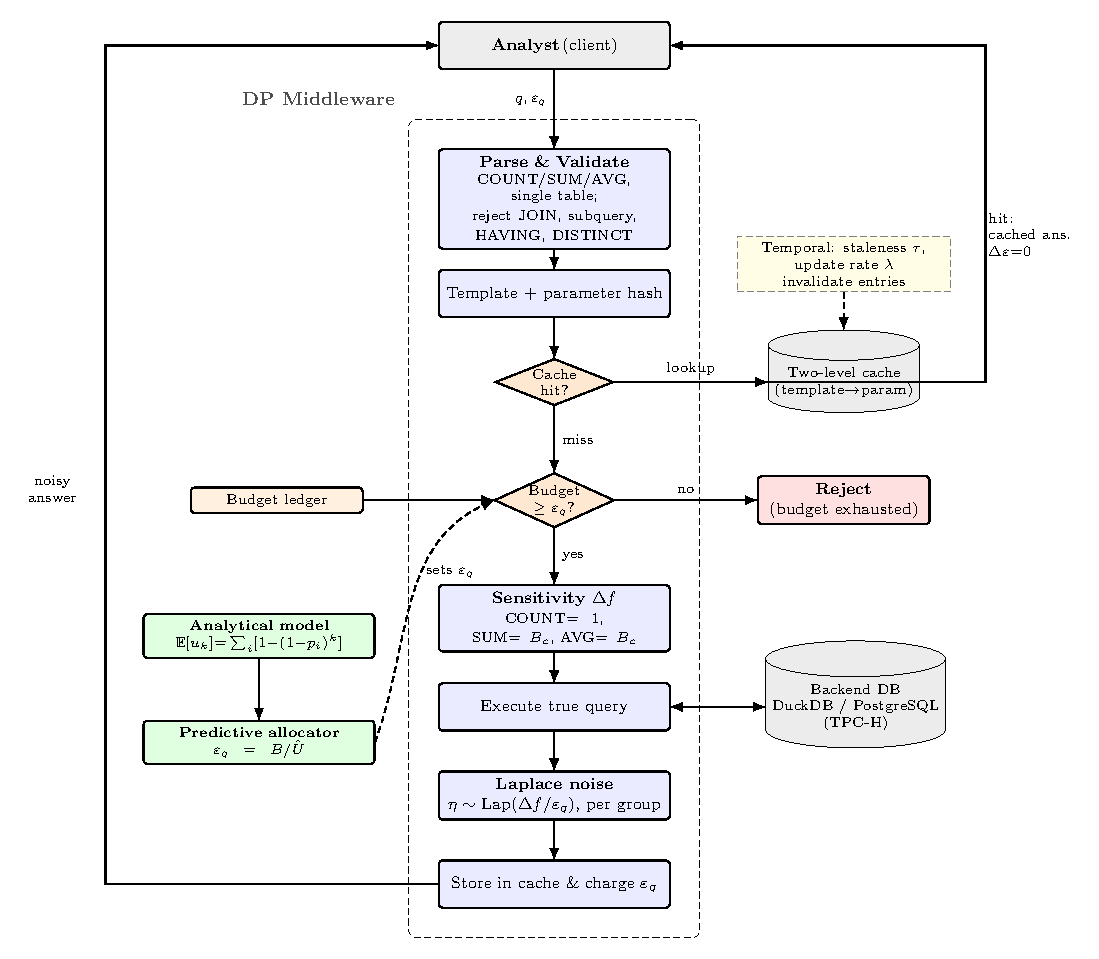
\includegraphics[width=\columnwidth]{fig_arch}
\caption{Workload-aware DP-SQL middleware. A cache hit is free by post-processing; a miss is charged $\eps_q$, noised, and cached. The analytical model drives the predictive allocator ($\eps_q{=}B/\hat U$), and a temporal regime $(\tau,\lambda)$ invalidates stale entries.}
\label{fig:arch}
\end{figure}

\begin{algorithm}[t]
\caption{Workload-aware DP middleware (one query).}
\label{alg:full}
\begin{algorithmic}[1]
\REQUIRE Query $q$, budget $\eps_q$, ledger $\mathcal L$, staleness $\tau$, update $(\lambda,q_{\mathrm{inv}})$
\STATE Parse/validate $q$; advance clock; invalidate each entry w.p.\ $\lambda q_{\mathrm{inv}}$
\STATE Compute template hash $h_T$, parameter hash $h_P$
\IF{$\mathcal L.\mathrm{cache}[h_T][h_P]$ fresh (age $\le\tau$)}
 \STATE \textbf{return} cached $\tilde r$ \hfill {\small (post-processing, $\Delta\eps{=}0$)}
\ENDIF
\IF{$\mathcal L.\mathrm{remaining}<\eps_q$} \STATE \textbf{return} \textsc{BudgetExhausted} \ENDIF
\STATE $\Delta f\gets$ sensitivity; $\mathcal L.\mathrm{consumed}\mathrel{+}=\eps_q$
\STATE $r\gets$ execute $q$; $\tilde r\gets r+\Lap(\Delta f/\eps_q)$ per aggregate, per group
\STATE Cache and \textbf{return} $\tilde r$
\end{algorithmic}
\end{algorithm}

A \emph{temporal extension} couples budget to time, since in deployment the two cannot be separated: data updates invalidate cached answers and freshness requirements force re-noising. This is a \emph{first-order} treatment, a planning estimate rather than a full model. A complete staleness/update theory (with re-release policies and a proper arrival process) is a study in its own right, which we leave to future work.

Within this first-order treatment we work with a temporal \emph{planning estimate}, which is neither a proven bound nor an equality: if every template were re-queried in every freshness window, the number of (re-)noisings per template would be $N=\max(1,\lceil T/\tau\rceil)+T\lambda q$, giving the first-order estimate $\E[\eps_{\mathrm{temp}}]\approx\eps_q\,\E[u_k]\,N$. Because $N$ assumes every template is re-issued in \emph{every} window---ignoring the actual arrival schedule---the estimate is conservative: across independently seeded trials it over-predicts the realized budget in every cell with active dynamics (at $\tau{=}10$ it predicts ${\approx}70$ vs.\ a realized ${\approx}38$; at $\lambda{=}0.2$, ${\approx}49$ vs.\ ${\approx}32$; Section~\ref{sec:results}), so we commit to the \emph{trend}. Under a \emph{specified} arrival model, moreover, this estimate is a proven \emph{upper} bound:
\begin{prop}[Temporal budget upper bound]\label{prop:tempbound}
If the query-arrival process is independent of the data-update process, updates arrive as a Poisson($\lambda$) process and invalidate each cache entry independently with probability $q$, and a stale ($\mathrm{age}>\tau$) or invalidated entry is re-noised on its next query, then
$\E[\eps_{\mathrm{temp}}(T)]\le\eps_q\,\E[u_k]\,N$ with $N=\lceil T/\tau\rceil+\lambda T q$.
\end{prop}
\begin{proof}
Per template, partition re-noisings into staleness- and update-driven. A staleness re-noising resets the entry's age, so at most $\lceil T/\tau\rceil$ occur. Each update-driven re-noising consumes a distinct invalidation event, so their number is at most the invalidations hitting the template, whose expectation is $\le\lambda Tq$. Summing over the (independent) appeared templates gives $\E[u_k]\,N$; multiply by $\eps_q$. \end{proof}
\noindent This holds for the Poisson model above, \emph{not} for every arrival process; we validate it---the bound holds in $12/12$ simulated cells, strict and conservative (realized/bound $0.15$--$0.57$) in the dynamic regime and tight (equality) in the static one. The only \emph{unconditional} hard ceiling remains naive composition, $k\eps_q$. Three regimes slide continuously: \emph{(a) static} ($\tau\to\infty,\lambda{=}0,N{=}1$) recovers Section~\ref{sec:model}; \emph{(b) bounded staleness} ($\tau$ finite, $\lambda{=}0$); \emph{(c) update-driven} ($\lambda{>}0$). On the implementation side, the prototype is unit-tested across parser validation, sensitivity, Laplace calibration, cache semantics, the model limits, the concentration bound, and temporal re-noising.

While the \emph{magnitude} estimate above is not an unconditional bound, the re-release \emph{policy} that consumes it admits one. The planning estimate prices a schedule; the question a custodian actually faces is whether re-noising can overrun $B$. It cannot, if releases are budget-gated:

\begin{prop}[Budget-aware re-release: a provable ceiling]
\label{prop:barr}
Fix a per-release cost $\eps_q$ and total budget $B$, and consider the policy that, at each freshness tick, re-noises a stale or update-invalidated template only while the remaining budget is $\ge\eps_q$, and otherwise serves the last cached answer. Then for \emph{any} freshness interval $\tau$ and \emph{any} update process (volatility $\lambda$), the cumulative spend never exceeds $B$, and the number of re-releases is exactly $\min\!\bigl(R,\lfloor B/\eps_q\rfloor\bigr)$, where $R$ is the number of refreshes the schedule requests.
\end{prop}
\begin{proof}
Each release decrements the remaining budget by $\eps_q$ and is issued only when the remaining budget is $\ge\eps_q$, so the remaining budget stays $\ge0$ and the cumulative spend is non-decreasing and bounded above by $B$. Once $\lfloor B/\eps_q\rfloor$ releases have been made the remaining budget is $<\eps_q$ and every further refresh is denied, giving the stated count. \end{proof}

\noindent This is a worst-case \emph{guarantee}: it holds for every arrival process, unlike the magnitude estimate, and it makes the refresh rate a budgeting decision rather than an unverified assumption. The guarantee also turns the refresh rate into a formal \emph{optimization} problem in the remaining budget \emph{and} the volatility $\lambda$. Consider minimizing the time-average staleness, which is proportional to the refresh interval $\tau$, subject to the re-release budget constraint $\eps_q\,u_k\bigl(\lceil T/\tau\rceil+\lambda T q\bigr)\le B$ (the $\lambda Tq$ term is the volatility-driven spend of Proposition~\ref{prop:tempbound}). The objective is monotone increasing in $\tau$ while the feasible set is monotone in $\tau$, so the optimum sits on the budget boundary:
\begin{equation*}
\tau^\star(\lambda)=\frac{T}{\,B/(\eps_q u_k)-\lambda T q\,},\qquad\text{valid when }\ \lambda T q<\tfrac{B}{\eps_q u_k}.
\end{equation*}
This is the budget- and volatility-aware optimal refresh: a shorter $\tau$ violates the budget (trips the gate, leaving late ticks stale), a longer one wastes affordable freshness, and a higher update rate $\lambda$ \emph{raises} $\tau^\star$ because updates already consume part of $B$. At $\lambda{=}0$ it recovers $\tau^\star=T u_k\eps_q/B$; once $\lambda T q\ge B/(\eps_q u_k)$ the update load alone exhausts the budget and no staleness-driven refresh is affordable (we verify $\tau^\star(\lambda)$ spends exactly $B$ at the boundary). The remaining open piece is the full accuracy theory of $\E[\eps_{\mathrm{temp}}]$ under a general renewal arrival process.

%% ============================================================
\section{Results and Findings}
\label{sec:results}

\noindent This section reports the empirical findings. The single most important result is the real-trace forecast of Section~\ref{sec:redbench}: predicting a workload's full distinct-query count, and hence its budget, from only its first half cuts the error by $45\%$ over the plug-in estimate. The synthetic campaign below first establishes the model's arithmetic and invariances before turning to that real-trace evidence.

The experimental campaign comprises six sweeps totaling $4{,}155$ trials ($\sim$$150{,}000$ queries) over Zipf workloads ($m{=}7$ Adult age-bands and TPC-H templates), four per-query budgets $\eps_q\in\{0.1,0.5,1,2\}$, lengths $k\in\{10,\dots,500\}$, and two data scales (TPC-H at scale factor (SF) 1 with 6M lineitem rows, and SF=10 with 60M). We compare internal execution modes under one identical middleware so that the algorithmic effect of workload-aware accounting is isolated; an end-to-end comparison against external prototypes would require query-rewriting integration, which we leave as future work.

\subsection{Validating the model}

The first validation checks the model's $\E[u_k]$ against measurement: Table~\ref{tab:validation} compares the closed form to the 30-trial empirical mean across the main grid, and agreement is within $<3\%$ in $21$ of $24$ cells; the three outliers ($3.5$--$8.6\%$) occur at high skew and small $k$, where $\E[u_k]$ is tiny and a $0.1$-unit deviation is a large relative error. The savings ratio $S(k)$, computed from measured budget, matches within $<2\%$ in $23/24$ cells.

\begin{table}[t]
\caption{Model vs.\ empirical $u_k$, Zipf ($m{=}7$, 30 trials/cell). Parentheses: signed relative error (\%).}
\label{tab:validation}
\centering\footnotesize
\setlength{\tabcolsep}{3.5pt}
\resizebox{\columnwidth}{!}{%
\begin{tabular}{c|cccc}
\toprule
$\alpha\backslash k$ & 10 & 25 & 50 & 100 \\
\midrule
0.0 & 5.50/5.53 ($-0.6$) & 6.85/6.77 ($1.2$) & 7.00/7.00 ($0.0$) & 7.00/7.00 ($0.0$) \\
0.5 & 5.30/5.23 ($1.3$) & 6.73/6.73 ($-0.1$) & 6.98/6.93 ($0.7$) & 7.00/7.00 ($0.0$) \\
1.0 & 4.73/4.70 ($0.6$) & 6.32/6.30 ($0.3$) & 6.88/6.90 ($-0.3$) & 7.00/7.00 ($0.0$) \\
1.5 & 3.98/3.87 ($2.8$) & 5.57/5.70 ($-2.3$) & 6.48/6.40 ($1.3$) & 6.91/6.93 ($-0.3$) \\
2.0 & 3.25/3.13 ($3.5$) & 4.64/4.70 ($-1.3$) & 5.69/5.73 ($-0.7$) & 6.50/6.43 ($1.1$) \\
3.0 & 2.19/2.07 ($5.7$) & 3.07/3.33 ($-8.6$) & 3.85/3.90 ($-1.3$) & 4.72/4.67 ($1.1$) \\
\bottomrule
\end{tabular}}
\end{table}

Beyond pointwise agreement, the predicted invariances and limiting behavior also hold empirically. The model's $\E[u_k]$ is structurally independent of $\eps_q$ (confirmed within $0.12$ units across $\eps_q\in\{0.1,0.5,1,2\}$) and of data scale: the same templates over a $10\times$ larger TPC-H database (60M rows) give identical empirical $\E[u_k]$ to within $0.034$ units, isolating workload structure from data scale. Pushing skew to $\alpha{=}10$ at $k{=}200$, predicted and empirical $\E[u_k]$ stay within $0.13$ units while $\E[u_k]$ itself varies by an order of magnitude, and $S(k)\to99.4\%$ recovers the $1-1/k$ corner numerically (Figure~\ref{fig:limits}).

\begin{figure}[h]
\centering
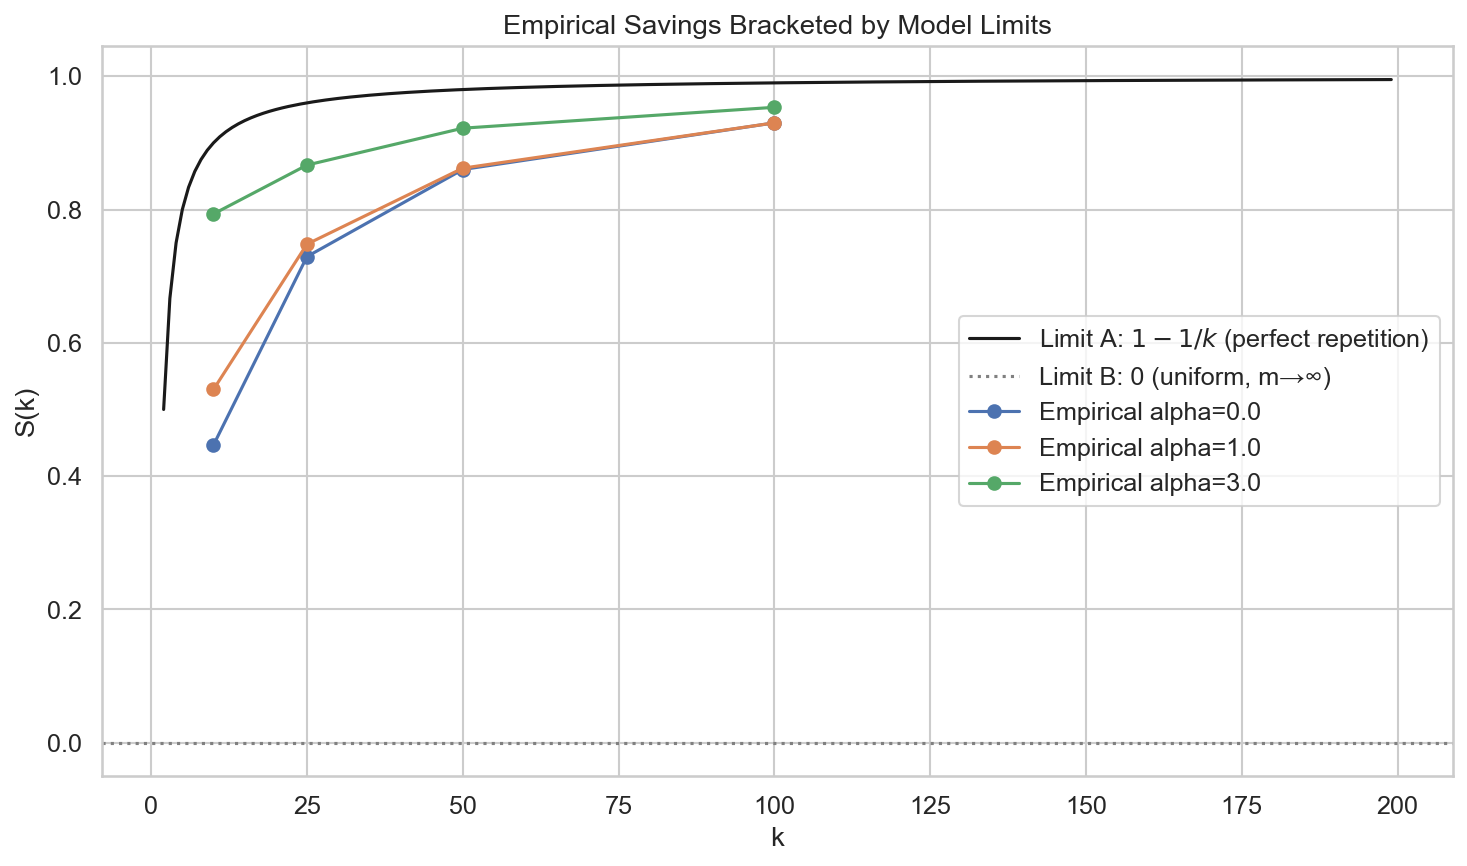
\includegraphics[width=0.92\columnwidth]{model_validation/model_validation_limits.png}
\caption{Savings ratio $S(k)$ vs.\ workload length, several Zipf $\alpha$. Dashed: model. Markers: empirical mean (30 trials). High-$\alpha$ curves approach $1-1/k$ (Limit~A); the $\alpha{=}0$ curve stays near $0$ until $k$ approaches $m$, then saturates (Limit~C, finite $m$).}
\label{fig:limits}
\end{figure}

The validation so far assumes i.i.d.\ arrivals. To probe the forecast's robustness to this assumption, we extend the occupancy model to correlated and non-stationary arrival processes, beginning with a bursty ``sticky'' process.
\begin{prop}[Sticky-Markov occupancy]\label{prop:sticky}
Under the sticky arrival process---$X_1\sim\{p_i\}$, and for $t\ge2$, $X_t{=}X_{t-1}$ with probability $s$ else a fresh draw $\sim\{p_i\}$ (a bursty workload with stationary marginal $\{p_i\}$)---the expected distinct count is
\[
\E[u_k]=\sum_i\Bigl[1-(1-p_i)\bigl(s+(1-s)(1-p_i)\bigr)^{k-1}\Bigr].
\]
\end{prop}
\begin{proof}
The set of distinct templates visited equals the set of distinct values among the \emph{fresh} draws (a repeat only re-emits the current template), and the number of fresh draws is $F=1+\mathrm{Binom}(k-1,1-s)$. Conditioning on $F$ and using $\E[z^{\mathrm{Binom}(n,1-s)}]=(s+(1-s)z)^n$ with $z=1-p_i$ gives the result. At $s{=}0$ it recovers the i.i.d.\ $\E[u_k]$; at $s{=}1$ it gives $1$. \end{proof}

\begin{prop}[General-Markov occupancy]\label{prop:markov}
For an \emph{arbitrary} Markov arrival process with transition matrix $P$ ($P[j,l]=\Pr[X_{t+1}{=}l\mid X_t{=}j]$) and initial law $\nu$, let $Q_i$ be the sub-stochastic block of $P$ on the states $\neq i$ and $\nu_i$ the initial mass on those states. Then
$\E[u_k]=\sum_i\bigl[1-\nu_i^{\!\top} Q_i^{\,k-1}\mathbf 1\bigr]$.
\end{prop}
\begin{proof}
State $i$ is unvisited iff the chain stays in $\{\cdot\neq i\}$ for all $k$ steps, an event of probability $\nu_i^{\!\top}Q_i^{\,k-1}\mathbf 1$; summing the complements over $i$ gives the result. The i.i.d.\ form (every row of $P$ equal to $\{p_i\}$) and the sticky form of Proposition~\ref{prop:sticky} are special cases. \end{proof}
\noindent This closes the occupancy model for \emph{any} Markovian arrival pattern; it reproduces both special cases to machine precision and matches simulation to $\le10^{-3}$ on random chains.

\begin{prop}[Latent-state (Markov-modulated) occupancy]\label{prop:hmm}
When the query distribution is itself non-stationary---a hidden Markov chain with transition matrix $T$ and initial law $\omega$ selects, in state $h$, an emission distribution $p^{(h)}$ over the templates---the expected distinct count is
\[
\E[u_k]=\sum_i\Bigl[1-\omega^{\!\top} D_i\,(T D_i)^{\,k-1}\mathbf 1\Bigr],\qquad D_i=\mathrm{diag}\bigl(1-p^{(h)}_i\bigr),
\]
where $D_i$ collects the per-state probabilities of \emph{not} emitting template $i$.
\end{prop}
\begin{proof}
Template $i$ is unvisited iff every step avoids it; weighting the hidden paths by their probability of avoiding $i$ gives $\omega^{\!\top}D_i(TD_i)^{k-1}\mathbf 1$, and summing the complements over $i$ gives $\E[u_k]$. A single hidden state recovers the i.i.d.\ form, and a deterministic emission ($p^{(h)}{=}e_h$) recovers Proposition~\ref{prop:markov}, and through it the sticky and i.i.d.\ cases. \end{proof}
\noindent This covers regime-switching workloads whose $\{p_i\}$ drifts with a latent state. On a two-regime chain, each regime concentrating on a different half of the templates, the closed form matches simulation to $\le0.03$, whereas a stationary i.i.d.\ forecast that ignores the regimes mis-predicts $u_k$ by up to $1.7$; the latent structure must therefore be modeled explicitly, which the proposition provides.

\noindent Across these robustness extensions, four properties make the forecast dependable. \emph{(i) Distribution-agnostic}: it is exact for any i.i.d.\ marginal (uniform, Zipf, lognormal-shaped), matching the empirical mean to $\le0.2$. \emph{(ii) Concentrated}: by Proposition~\ref{prop:conc} the standard deviation is small, $\sqrt V{=}0.11$--$1.77$ at $m{=}20$, so the spread around the forecast is tight. This is a variance- or Chebyshev-scale statement, not a high-probability envelope. \emph{(iii) Exact on heterogeneous workloads}: on a constructed mixed W1+W4 workload with true $u_k=1+(1-f)k$, the closed form $\eps_q u_k$ matches the measured budget exactly at every mixing fraction (Table~\ref{tab:mixed}). \emph{(iv) Conservative under \emph{positive} correlation}: a bursty sticky-Markov process (the tested case; same stationary marginal) clusters repeats and lowers the distinct count, so the i.i.d.\ forecast \emph{over}-predicts $u_k$ by $1.09$/$1.29$/$2.72\times$ at stickiness $s{=}0.3$/$0.6$/$0.9$---the safe direction. This over-prediction is now \emph{exact}: Proposition~\ref{prop:sticky} gives the sticky-process $\E[u_k]$ in closed form (matching simulation to $<0.08$ across $16$ cells)---extending the occupancy model from i.i.d.\ to a Markovian arrival process---and the i.i.d.\ forecast is its $s{=}0$ special case, exceeding it for $s{>}0$, so the burstiness gap is quantified exactly rather than merely bounded by $u_k\le m$. The conservative-direction guarantee holds only for this positive-correlation process. Anti-correlated or without-replacement arrivals would instead push $u_k$ above i.i.d.\ and make the forecast optimistic. The unconditional safety net is therefore the $\eps_q{=}B/m$ allocator: in the \emph{static} regime $u_k\le m$ for any arrival process, so it never rejects (under temporal re-noising the same query can be charged again, so this becomes a per-window guarantee).

\begin{table}[h]
\caption{Mixed W1+W4 workload, $B{=}50$, $\eps_q{=}0.5$, 20 trials. The closed form matches the measured budget exactly.}
\label{tab:mixed}
\centering\small
\begin{tabular}{c|c|cc}
\toprule
$f$ & true $u_k$ & measured $\eps$ used & predicted $\eps_q u_k$ \\
\midrule
0.1 & 91 & 45.5 & 45.5 \\
0.3 & 71 & 35.5 & 35.5 \\
0.5 & 51 & 25.5 & 25.5 \\
0.7 & 31 & 15.5 & 15.5 \\
0.9 & 11 & 5.5 & 5.5 \\
\bottomrule
\end{tabular}
\end{table}

The temporal extension of Section~\ref{sec:system} is validated in the same manner: we sweep $\tau$ (with $\lambda{=}0$) and $\lambda$ (with $\tau$ large), over independently seeded trials so each draws an independent update stream. The planning estimate $\eps_q\E[u_k]N$ tracks the empirical mean in trend and matches at large $\tau$ (rare re-noising); in every cell with active dynamics it \emph{over}-predicts the realized budget (at $\tau{=}10$, ${\approx}70$ vs.\ an empirical ${\approx}38$; at $\lambda{=}0.2$, ${\approx}49$ vs.\ ${\approx}32$), since not all re-noisings materialize within the horizon. Under the Poisson update model of Proposition~\ref{prop:tempbound} it is moreover a proven \emph{upper} bound, which we confirm holds in $12/12$ simulated cells; for an unspecified arrival process we report it as a conservative planning estimate. In both regimes, freshness carries an explicit, bounded cost.

\subsection{Real-workload validation (Redbench)}
\label{sec:redbench}

The synthetic sweep cannot establish \emph{external} validity, so we add the first test on production-derived traces: Redbench~\cite{redbench2025}, 30 analytical SQL workloads synthesized from Amazon Redshift's Redset query log, in which each user's real query timeline (and thus its repetition structure) is mapped onto CEB+/JOB query instances. Redbench is \emph{not} a differential-privacy benchmark; we use its production-derived query-repetition structure solely to externally validate our workload-occupancy forecast, not any DP mechanism of its own. The exact-query identity is the SQL instance, so Redbench's own \emph{query-repetition rate} $=1-u_k/k$, computed from the realized distinct count $u_k$, is exactly our $S(k)$. Running the occupancy model against all 30 workloads yields five findings.
\emph{(1) Real workloads span the full skew range:} realized $S(k)$ runs from $0\%$ to $98\%$ (mean $53\%$), so template repetition (the structure the model exploits) is pervasive in production rather than an artifact of the sweep.
\emph{(2) Real distributions are heavy-tailed:} fitting Zipf to each workload gives $\alpha\in[0,3]$ with mean $0.84$ (near classic Zipf), and our synthetic sweep $\alpha\in\{0,\dots,3\}$ \emph{brackets} the real range, which grounds the Zipf parameterization of the synthetic sweep in production data.
\emph{(3) The descriptive fit is tight:} when fed the full-trace $\{p_i\}$, the closed form reproduces the realized savings to a mean absolute $0.13$ in $S(k)$---but this is an \emph{in-sample, descriptive} check (it uses the whole trace), not a before-execution forecast.
\emph{(4) The before-execution forecast succeeds} (our headline real-data result): estimating $\{p_i\}$ from only the \emph{first $50\%$} of each timeline and predicting the full $u_k$, the smoothed Good--Toulmin estimator~\cite{orlitsky2016unseen} cuts the plug-in's error by $45\%$ ($0.22\!\to\!0.12$ in $u_k/k$). The \emph{plug-in} simply assumes the rest of the workload repeats the query mix seen so far, whereas the \emph{Good--Toulmin} (unseen-species) estimator also predicts how many \emph{brand-new} queries are still to come, the classic ``how many species have we not yet seen?'' problem, so it forecasts $u_k$ more accurately from a short prefix. This is the genuine forecast rather than the in-sample fit, and on production-derived data it confirms that unseen-species correction is the right tool. Redbench is trace-\emph{derived} synthesis (real repetition structure, CEB+/JOB queries, not raw production SQL), so it raises external validity substantially without fully eliminating the gap (Section~\ref{sec:discussion}).
\emph{(5) The forecast survives a controlled out-of-distribution check:} to rule out that it is an artifact of the Zipf self-consistency setup, we run the \emph{same} prefix-forecaster on synthetic workloads drawn from five families it is never told about---two Zipf, plus uniform, lognormal-shaped, and a heavy Pareto tail. Forecasting the full $u_k$ from a $50\%$ prefix, the smoothed Good--Toulmin estimator stays within a mean $0.021$ (max $0.026$) in $u_k/k$ across \emph{all five}, Zipf and non-Zipf alike, cutting the naive prefix-distinct error by $76\%$: the forecast is not tied to the Zipf assumption. Beyond horizon $t{=}(k{-}n)/n\approx1$ (e.g.\ a $25\%$ prefix) the unseen-species series degrades, as is well known for Good--Toulmin, so we clamp the estimate to $[D_n,k]$ (a distinct count cannot exceed $k$), which turns any divergence into the budget-safe over-forecast.

\subsection{Budget savings and where naive composition fails}

The budget savings themselves follow the model's predictions. Across the full grid of six workloads, workload-aware accounting answers the same $100$ queries at comparable per-query MAE while spending only $\eps_q u_k$: savings of $100\times$ on the repetitive W1, then $33\times$, $20\times$, and $14.3\times$ on the TPC-H and uniform pools (where $u_k$ saturates at the pool size $m$), and \emph{exactly} $1\times$ on the genuine drill-down W4, where every query is unique and the model correctly predicts $S(k){=}0$ (Table~\ref{tab:fullgrid}, Figure~\ref{fig:savings}). These multipliers are accounting ratios $1/(1-S(k))$ that any exact-repeat cache attains; our contribution is the closed-form \emph{prediction} of $S(k)$ before execution (within $<3\%$), not the saving itself.

\begin{table}[h]
\footnotesize\centering
\caption{Full grid (6 workloads, $k{=}100$, $\eps_q{=}1$, 30 trials). Workload-aware spends $\eps_q u_k$ at $93$--$99\%$ cache-hit rates; the drill-down (W4) is the predicted no-win case.}
\label{tab:fullgrid}
\begin{tabular}{l|cc|c}
\toprule
Workload & naive $\eps$ & work.-aware $\eps$ & savings \\
\midrule
W1 Repetitive & 100.0 & 1.0 & $100\times$ \\
W2 TPC-H returnflag & 100.0 & 3.0 & $33\times$ \\
W2 TPC-H priority & 100.0 & 5.0 & $20\times$ \\
W2 Zipf $\alpha{=}1$ & 100.0 & 7.0 & $14.3\times$ \\
W3 Uniform & 100.0 & 7.0 & $14.3\times$ \\
W4 Drill-down (unique) & 100.0 & 100.0 & $1\times$ \\
\bottomrule
\end{tabular}
\end{table}

\begin{figure}[h]
\centering
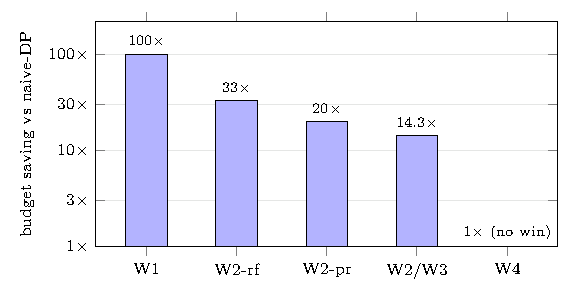
\includegraphics[width=0.92\columnwidth]{fig_savings}
\caption{Budget saved vs.\ naive ($k{=}100$, $\eps_q{=}1$, log scale): up to $100\times$ on the repetitive W1 and $14$--$33\times$ on the parametric/uniform pools, but exactly $1\times$ (no win) on the unique drill-down W4---the model predicts the $S(k){=}0$ case rather than overclaiming.}
\label{fig:savings}
\end{figure}

Two concrete failure regimes of naive composition sharpen this comparison. On the real middleware (Adult, $B{=}10$, $k{=}100$, 12 trials; Table~\ref{tab:killer}), repetition turns the structural advantage into a stark gap. \emph{(A) Budget exhaustion}: a dashboard re-issuing one tile at fixed $\eps_q{=}1$ exhausts naive after $B/\eps_q{=}10$ queries ($10/100$ answered), while caching answers all $100/100$ for free---a $10\times$ gap. \emph{(B) Accuracy at fixed total budget}: to answer all $100$, naive must thin the budget ($\eps_q{=}B/k{=}0.1$, error $\approx10$), whereas concentrating it on the $u_k{=}1$ distinct release makes the answer almost exact. \emph{(C) Control}: on a genuine drill-down both modes match at error $\approx9.6$; we include this case because the model predicts it to be the no-win case.

\begin{table}[h]
\footnotesize\centering
\caption{Naive's failure regimes vs.\ workload-aware (real middleware, Adult, $B{=}10$, $k{=}100$).}
\label{tab:killer}
\begin{tabular}{l|cc|cc}
\toprule
& \multicolumn{2}{c|}{Naive} & \multicolumn{2}{c}{Workload-aware} \\
Workload & ans. & $|$err$|$ & ans. & $|$err$|$ \\
\midrule
Repetitive, fixed $\eps_q{=}1$ & $10/100$ & $0.9$ & $\mathbf{100/100}$ & $0.4$ \\
Repetitive, fixed budget $B$ & $100/100$ & $10.0$ & $100/100$ & $\mathbf{\approx0}$ \\
Drill-down (all unique) & $100/100$ & $9.6$ & $100/100$ & $9.6$ \\
\bottomrule
\end{tabular}
\end{table}

\subsection{Predictive allocation}

The validated model is not only descriptive but also \emph{prescriptive}: an allocator estimates $\hat U=\E[u_k]$ online (after a short warmup) and sets $\eps_q=B/\hat U$ to target the offline optimum $\eps_q^*=B/u_k$ \emph{under a uniform per-distinct-release objective} (a frequency-/importance-weighted error tilts $\eps$ toward the frequent templates---Appendix~\ref{app:identifiability}), capping spend at $B$. At a fixed \emph{total} budget this trades coverage for accuracy: on Zipf workloads ($k{=}100$, $B{=}10$) it lowers per-query MAE on the \emph{answered} subset (Table~\ref{tab:predictive}; it answers $69$--$88/100$ where naive answers $100$) by $16.8\%$ ($\alpha{=}0$) down to $5.4\%$ ($\alpha{=}2$). The gain is only \emph{borderline} (paired $t$-test $p\approx0.05$ at $\alpha{=}0$, not crossing $0.05$; $p>0.3$ for $\alpha\ge1$); the improvement is directional rather than uniform, and it is bought with late-query rejections. The robust result is instead the \emph{safe} allocator $\eps_q{=}B/m$, which never rejects in the static regime ($u_k\le m$; temporal re-noising can charge the same query again) and matches a learned bandit's best operating point at zero exploration cost, as the next comparison details.

A practical comparison places the safe allocator against a learned baseline. Against an $\eps$-greedy learned bandit that must \emph{explore} to find a good per-query $\eps$, the closed-form safe allocator $\eps_q{=}B/m$ reaches the bandit's best operating point at \emph{zero} exploration cost: on the Zipf allocation benchmark it attains per-release MAE $2.0$ versus the bandit's $3.6$ at the same answer rate, because the forecast hands the allocator $\hat U$ directly instead of learning it online through trial releases. The bandit's own arm set includes the $B/m$ denominator, so the closed form supplies, without exploration, the operating point the bandit must otherwise pay to find. This result shows the closed form reaching the bandit's operating point at zero cost rather than beating it, and the safe allocator's advantage narrows for $m{>}k/4$ where $B/m$ is no longer the best arm. The budget sweep ($32\%$ savings at $B{=}1$, growing with $B$) and scale-invariance ($40\%$ at SF$=10$) show the allocator is not tuned to a single operating point. The estimate $\hat U$ is produced by an online \emph{workload-learning} step---a Laplace-smoothed empirical $\{p_i\}$ refined by the smoothed Good--Toulmin unseen-species correction (Section~\ref{sec:redbench})---which already generalizes across distribution families (finding~5) and over real Redbench traces. The full head-to-head, the learned-bandit curves, and the predictive ablation are in Appendix~\ref{app:allocator}.

The forecast must also remain accurate under workload drift: the $\{p_i\}$ a deployment learns online need not be stationary, and a system that re-estimates it should track change. We therefore add a drift-aware streaming learner, an exponentially weighted moving average (EWMA) that decays stale template mass and re-centers $\hat U$ on the current regime. On a workload whose distribution \emph{shifts} mid-stream it tracks the post-shift horizon about $15\times$ more accurately than a non-forgetting full-history plug-in. It is a planning-layer estimator, so privacy still rests on the public cap $m$ and the ledger; the latent-state occupancy of Proposition~\ref{prop:hmm} is the matching closed-form forecast for such regime-switching streams.

\begin{table}[h]
\footnotesize\centering
\caption{Predictive allocator vs.\ fixed-$\eps_q$ baselines (mean $\pm$ standard error (SE), 30 trials, $k{=}100$, $B{=}10$). MAE is over answered queries; the allocator answers fewer (69--88) than naive (100). The gain is borderline ($p\approx0.05$) only at $\alpha{=}0$.}
\label{tab:predictive}
\begin{tabular}{c|l|ccc}
\toprule
$\alpha$ & Mode & MAE & answered & $\eps$ spent \\
\midrule
\multirow{2}{*}{0.0} & Naive & 9.86 & 100/100 & 10.0 \\
 & \textbf{Predictive} & \textbf{8.21}$\pm$0.85 & 69/100 & 10.0 \\
\midrule
\multirow{2}{*}{1.0} & Naive & 9.81 & 100/100 & 10.0 \\
 & \textbf{Predictive} & \textbf{8.98}$\pm$0.93 & 78/100 & 10.0 \\
\midrule
\multirow{2}{*}{2.0} & Naive & 9.96 & 100/100 & 10.0 \\
 & \textbf{Predictive} & \textbf{9.42}$\pm$1.40 & 88/100 & 10.0 \\
\bottomrule
\end{tabular}
\end{table}

To place these results against prior systems, we frame the comparison as concrete situations a custodian faces; on the raw savings numbers we are level with prior work rather than ahead of it. Before any query executes, the forecast supplies a $t{=}0$ completion check (a hard yes under $B/m$, since $u_k\le m$) and a \emph{per-release} $(\alpha,\beta)$ accuracy verdict (Appendix~\ref{app:apriori}), plus capacity planning from a prefix (the $45\%$ Redbench result); reactive systems surface these only by spending budget query-by-query. On the savings \emph{number} itself we do not lead: we cite the baselines' own published figures rather than re-running them (Turbo $1.7$--$15.9\times$~\cite{kostopoulou2023turbo}, CacheDP a reduction under an accuracy contract~\cite{mazmudar2023cachedp}) against our $14$--$33\times$ on the pools and $100\times$ on pure repetition: the same order of magnitude, so we claim \emph{parity}, not superiority (the workloads and mechanisms differ, so this is a ballpark placement, not a controlled run). A controlled, same-hardware comparison was not feasible within this study: the implementation of the academic PrivateSQL prototype was never publicly released (the paper, of course, is public) and Chorus is no longer maintained, while Turbo and the CacheDP research artifact are available but expose linear-query interfaces to which our SQL workloads would first have to be ported---the concrete head-to-head we identify in Section~\ref{sec:future}. At a fixed budget the safe $\eps_q{=}B/m$ allocator simply \emph{reaches} an $\eps$-greedy bandit's best operating point at zero exploration cost, as shown above (Appendix~\ref{app:allocator}). The contribution is the \emph{before-execution} deliverable the others lack, not a larger multiplier.

\subsection{Privacy leakage}

We next verify that the accounting does not weaken the privacy guarantee itself: two attacks confirm the per-query calibration. \emph{Membership inference}: an adversary observing one noisy COUNT must decide whether a target is present. The optimal single-release attacker's \emph{accuracy} is bounded by $e^\eps/(1+e^\eps)$; the empirical area under the ROC curve (AUC)---which for this symmetric single-release threshold test nearly equals the attacker's accuracy---stays at or below that bound (within $\le1\%$) and is at chance for $\eps\le0.1$ (Table~\ref{tab:leak}, left). A fully type-matched comparison would use the exact Laplace AUC; the two nearly coincide here. \emph{Reconstruction}: replaying a 5-level differencing drill-down on real Adult counts $(48842,34327,24137,7210,3137)$, the mean absolute error scales as $1.5/\eps$, the expected absolute difference of two $\Lap(1/\eps)$ variables, to within a few percent across three orders of magnitude (Table~\ref{tab:leak}, right, indexed by the \emph{per-release} $\eps$). The attack is \emph{five} releases, so by sequential composition it costs a \emph{cumulative} $5\eps$; at a fixed total budget $B$ the per-release value is $\eps{=}B/5$ and the error scales accordingly: the Dinur--Nissim view ties reconstruction to the total budget spent, not the per-query value. (A stronger shadow-model membership inference attack (MIA) at our sample size was inconclusive, a negative result that we report in the artifact rather than as a leakage claim.) Our calibration conclusion rests on the clean single-query MIA and the reconstruction above, both of which degrade exactly where the model predicts efficient budgeting (high skew, low $\eps_q$); the reconstruction in particular succeeds on the W4 drill-down, which the model flags as the no-savings case.

\begin{table}[h]
\footnotesize\centering
\caption{Leakage vs.\ per-release $\eps$. Left: single-release membership-inference AUC vs.\ the DP \emph{accuracy} bound $e^\eps/(1+e^\eps)$ (AUC$\approx$accuracy for this symmetric test). Right: differencing reconstruction error vs.\ the $1.5/\eps$ reference (a 5-release attack; cumulative cost $5\eps$).}
\label{tab:leak}
\begin{tabular}{c|cc||c|cc}
\toprule
$\eps$ & AUC & $\frac{e^\eps}{1+e^\eps}$ & $\eps$ & rec.\ err & $1.5/\eps$ \\
\midrule
0.01 & 0.499 & 0.503 & 0.01 & 148.2 & 150.0 \\
0.10 & 0.522 & 0.525 & 0.10 & 14.8 & 15.0 \\
1.00 & 0.724 & 0.731 & 1.00 & 1.5 & 1.5 \\
5.00 & 0.988 & 0.993 & 5.00 & 0.3 & 0.3 \\
\bottomrule
\end{tabular}
\end{table}


\subsection{Runtime and overhead}

Finally, we quantify the runtime overhead: the privacy machinery is cheap relative to I/O. Across $1{,}500$ instrumented queries, cache hits are $2.7\times$ faster than misses ($0.76$ vs.\ $2.02$ ms) because they skip the database round-trip (36\% of miss cost); SQL parsing is 21\%, and the privacy-specific stages (sensitivity, allocation, noise) sum to under $0.25$ ms. Tail latency is controlled (miss $p99{=}5.1$ ms, hit $p99{=}3.6$ ms), and single-threaded throughput is $\sim$$495$ q/s on the miss path and $\sim$$1{,}320$ q/s on the hit path, so a workload-aware mode running at a $93$--$99\%$ hit rate sustains analyst-tier load. The asymptotic cost of the forecast itself is $O(m)$ per evaluation of $\E[u_k]$. A separate end-to-end measurement against raw DuckDB on \emph{identical} SQL quantifies the practical-system overhead the deployed comparison demands: the full DP miss path adds roughly $2$--$6\times$ over a bare query (sub-millisecond to ${\sim}1.2$ ms; hardware-dependent), an $\eps{=}0$ cache hit is ${\sim}5\times$ faster (${\sim}0.2$--$0.3$ ms) and free in budget, and a mixed repeated workload sustains ${\sim}1.4$--$1.6$k queries/s at a ${\sim}74\%$ hit rate; the workload-aware DP middleware is therefore practical as a deployed layer.

In interpreting these results, the two validations should be weighed differently: the synthetic grid (the $<3\%$ agreement) is a \emph{self-consistency} check---it confirms the estimator's arithmetic, not that real workloads are i.i.d.\ Zipf---whereas the genuine external evidence is the Redbench prefix forecast, a $45\%$ error reduction on traces the model never saw. Between the two sits the controlled out-of-distribution test (Section~\ref{sec:redbench}, finding~5): the deployable prefix-forecaster predicts $u_k$ within $\approx2\%$ on uniform, lognormal, and Pareto workloads it was never told the family of, so the headline accuracy is not an artifact of drawing the workload from the same Zipf the closed form integrates.

%% ============================================================
\section{Beyond Single-Table Aggregates: Multi-Table Joins}
\label{sec:joins}

A natural objection is that our closed-form models were derived for single-table COUNT/SUM/AVG, where the sensitivity $\Delta f$ is a public constant ($1$ for COUNT, the column bound $B_c$ for SUM/AVG; Section~\ref{sec:prelim}), and that they break for multi-table JOINs, whose sensitivity analysis is notoriously harder. This section separates the part that transfers unchanged from the part that genuinely degrades, and \emph{measures} the transfer on a real TPC-H join (Figure~\ref{fig:joins}).

\begin{prop}[Mechanism-agnostic forecast]
\label{prop:agnostic}
The expected distinct count $\E[u_k]$, the savings $S(k)=1-\E[u_k]/k$, the workload-aware spend $\eps_q\E[u_k]$, and the relative utility ratio $k/\E[u_k]$ are functions of $(m,\{p_i\},k)$ alone; they are invariant to the per-query DP mechanism and to its sensitivity $\Delta f$, and therefore transfer from single-table aggregates to any query class---joins included---unchanged.
\end{prop}
\begin{proof}
Each is built from $\E[u_k]=\sum_i[1-(1-p_i)^k]$ (Prop.~\ref{prop:eu}), a function of the arrival distribution only; $\Delta f$ enters solely the noise scale $\Lap(\Delta f/\eps_q)$ and cancels in the ratio $k/\E[u_k]$. \end{proof}

\noindent The single-table results of this paper are then the $d_{\max}{=}1$ instance of the join-parameterized framework below.

What transfers is the entire forecasting layer, because it reads the \emph{query stream} alone: $\E[u_k]$ (Prop.~\ref{prop:eu}), the savings $S(k)$ (Prop.~\ref{prop:savings}), the limiting behavior, the skew-monotonicity (Prop.~\ref{prop:zipf}), the concentration bound (Prop.~\ref{prop:conc}), and the spend $\eps_q\E[u_k]$ depend on $(\{p_i\},k,m)$ alone, never on what a query computes or how sensitive it is. Three quantities therefore transfer to a JOIN workload \emph{unchanged}. The \emph{spend} forecast holds because an exact JOIN repeat is still served free as post-processing; the \emph{relative utility} ratio $k/\E[u_k]$ holds because $\Delta f$ cancels, so it stays before-execution even when $\Delta f$ is unknown; and \emph{budget completion} holds because the $\eps_q{=}B/m$ ledger never overruns, since $u_k\le m$ is purely combinatorial. What does \emph{not} transfer for free is \emph{answerability}. A general equi-join has unbounded global sensitivity, so a usable $\eps_q$-DP answer needs a finite per-template sensitivity bound, and the \emph{absolute} per-release $(\alpha,\beta)$ verdict, which reads $\Delta f$ directly, inherits whatever that bound costs.

The one input that does change when moving to joins is the noise calibration, the scale $\Lap(\Delta f/\eps_q)$: adding one tuple to $R$ in $R\bowtie S$ can match arbitrarily many tuples in $S$, so the worst-case global sensitivity is unbounded and textbook Laplace calibration is undefined. The literature replaces the global constant with an instance-dependent or relaxed bound: smooth sensitivity~\cite{nissim2007smooth}, elastic sensitivity (FLEX), an efficiently computable bound from per-attribute max-frequencies~\cite{johnson2018towards}, residual sensitivity for multi-way self-join-free counts~\cite{dong2021residual}, and R2T, which truncates each entity's contribution at a privately chosen threshold and is the first to handle foreign keys (FK) with self-joins~\cite{dong2022r2t}. None of these is a drop-in replacement: the smooth-sensitivity route generally costs an $(\eps,\delta)$ relaxation, and R2T spends budget to pick $\tau$ and injects clipping bias. The conservative public route we adopt is a declared foreign-key multiplicity $d_{\max}$ (TPC-H caps line-items-per-order at $7$, so $d_{\max}{=}7$): capping makes $\Delta f{=}d_{\max}$ a public global-sensitivity constant, the $B_c$-style bound we already use for SUM/AVG and looser than the instance-optimal options. The join COUNT is then calibrated with $\Lap(d_{\max}/\eps_q)$, and the occupancy/spend forecast and $B/m$ sizing apply unchanged. The cache, the distinct-release count, and the $O(m)$ forecast cost are untouched; only the ledger semantics (pure $\eps$ vs.\ $(\eps,\delta)$) and the absolute accuracy verdict are. Self-joins are the genuinely hard regime, since one entity can raise many others' degrees, which is exactly what R2T targets.

We confirm the preceding analysis empirically on TPC-H by running the worked example as a \emph{twin} experiment: one Zipf identity stream over the $m{=}5$ order-priority pool, instantiated both as the single-table COUNT ($\Delta f{=}1$) and as the \texttt{orders}$\bowtie$\texttt{lineitem} COUNT ($\Delta f{=}d_{\max}{=}7$) on the real $1.5$M-order / $6$M-line-item tables ($600$ trials, $\alpha\in\{0,\dots,2\}$, $k\in\{10,\dots,100\}$). Confirming Proposition~\ref{prop:agnostic}, the forecast is \emph{identical} on the two sides: the realized distinct count, $\E[u_k]$, the savings $S(k)$, and the spend $\eps_q u_k$ coincide trial-for-trial, since occupancy reads only the identity stream. It tracks the closed form within $1.4\%$ on average ($17/20$ cells under $3\%$, the same accuracy as the single-table grid; Figure~\ref{fig:joins}, left). The \emph{only} quantity that moves is the per-release noise: the answered-release MAE is $7.6\times$ larger on the join side (Figure~\ref{fig:joins}, right), matching the $d_{\max}{=}7$ sensitivity ratio (expected exactly $7$; the small excess is finite-sample mean-absolute noise over the few answered releases), while the relative utility ratio $k/\E[u_k]$ is unchanged because $\Delta f$ cancels. The sensitivity-agnostic transfer is thus measured rather than merely argued: the closed-form forecast holds on a real multi-table join exactly as on the single table, and the join's added difficulty is confined to the orthogonal per-release $\Delta f$.

Beyond the offline twin experiment, the middleware also \emph{executes} the FK join end-to-end under DP, so the transfer is a property of the running system rather than only of the analysis. A single two-table inner equi-join \texttt{COUNT} parses, is charged the public FK-multiplicity sensitivity $\Delta f{=}d_{\max}$ (the privacy unit is the parent entity, so removing one order removes up to $d_{\max}$ joined rows), is served the conservative $\Lap(d_{\max}/\eps_q)$ noise, and has its exact repeats hit the cache for $\eps{=}0$. This is the \emph{same} workload-aware ledger as the single-table path, with only $\Delta f$ changed. The unsafe envelope is rejected \emph{before} any budget is spent: \textsc{outer}/\textsc{cross} joins, queries with more than one join, \textsc{sum}/\textsc{avg} over a join, and any join whose $d_{\max}$ is not a declared public schema constant (whose global sensitivity would otherwise be unbounded). An end-to-end check confirms the live \texttt{orders}$\bowtie$\texttt{lineitem} COUNT runs with $\Delta f{=}7$, returns $\sim\!4\times$ the single-table count, caches repeats for free, and refuses every unsafe form; the behavior is covered by the unit-test suite of $233$ tests (no regressions), including the budget-aware re-release ceiling of Proposition~\ref{prop:barr} and the brute-force soundness of the equivalence-checked cache. The contribution is therefore more than a purely analytical wrapper: the before-execution forecast and the join transfer are both realized in a running, tested DP-SQL system.

Finally, because the public $d_{\max}$ clamp is deliberately conservative, we also implement an instance-optimal, data-dependent sensitivity bound computed at runtime and quantify its effect on the forecast. Following FLEX~\cite{johnson2018towards}, the elastic sensitivity of the equi-join COUNT is $\mathrm{ES}(0)=\max(\mathrm{mf}_L,\mathrm{mf}_R)$, where $\mathrm{mf}_L$ and $\mathrm{mf}_R$ denote the maximum join-key frequencies of the left and right relations, computed from the data at \emph{runtime}; its smooth version yields an $(\eps,\delta)$ noise scale. We verify by brute force over $50$k constructed join instances that $\mathrm{ES}(0)$ upper-bounds the true local sensitivity, so the mechanism is sound. For forecasting, the key observation is that the occupancy and spend are sensitivity-agnostic (Proposition~\ref{prop:agnostic}): the forecast is \emph{identical} whether the noise uses the public $d_{\max}$ or the runtime elastic bound, since only the per-release noise scale moves, not $u_k$. Consequently, the before-execution budget forecast stays exact even when the per-release noise is determined from the data at runtime. We confirm this directly: across a twin sweep the forecast quantities ($\E[u_k]$, $S(k)$, and the spend) are identical in every cell under the public $d_{\max}$ and the runtime elastic calibration, while only the per-release noise scale moves. The utility effect is local: on TPC-H \texttt{orders}$\bowtie$\texttt{lineitem} the elastic bound coincides with $d_{\max}{=}7$ (the realized max-frequency already equals the public cap, so there is nothing to gain), whereas on a join whose realized degree sits well below its public bound, such as \texttt{part}$\bowtie$\texttt{lineitem} (frequency $57$ against a clamp above $114$), it cuts the noise. Wiring residual sensitivity~\cite{dong2021residual} or R2T~\cite{dong2022r2t} for multi-way and self-joins is the natural next mechanism; the forecast layer needs no change for any of them.

\begin{figure}[t]
\centering
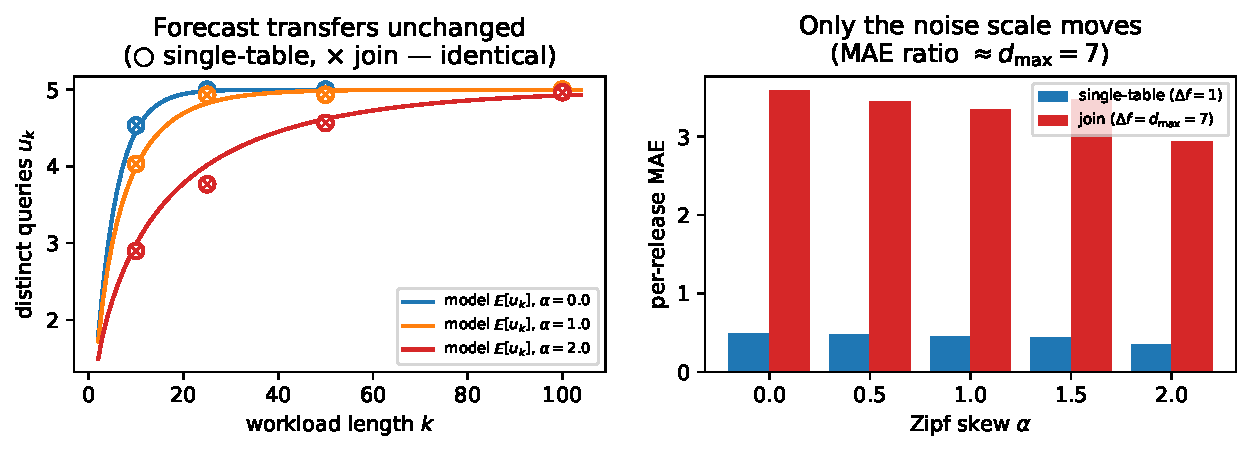
\includegraphics[width=\columnwidth]{fig_joins}
\caption{Twin single-table vs.\ join experiment (TPC-H, $m{=}5$ priority pool, $d_{\max}{=}7$, $600$ trials). \emph{Left:} the realized distinct count for the single-table ($\circ$) and join ($\times$) workloads lands on the \emph{same} analytical $\E[u_k]$ curve---the forecast transfers unchanged. \emph{Right:} only the per-release noise scale moves, by $\Delta f$ ($1$ vs $d_{\max}{=}7$).}
\label{fig:joins}
\end{figure}

%% ============================================================
\section{Limitations and Open Challenges}
\label{sec:future}
Rather than listing extensions, we pair each remaining limitation with the research problem it raises and a plausible path forward.

\subsubsection*{From repetition structure to linear structure}
The deepest limitation is the unit of accounting itself. Throughout this paper a query is either a repeat of an earlier one (free), a provably equivalent rewriting of one (free, Section~\ref{sec:model}), or entirely new (charged in full). Real analytical workloads, however, \emph{overlap} without being equivalent: range predicates nest, rollups aggregate the same cells at coarser granularity, and sliding windows shift by one bucket. Our forecast cannot price this overlap---two overlapping range counts form two equivalence classes and are charged twice, although much of the second answer is already determined by the first. This raises the central open problem: extending before-execution budget forecasting from \emph{repetition} structure to \emph{linear} structure. The natural formalization treats each aggregate as a linear query over a binned data vector $x$, so a workload of $k$ queries is a matrix $W_k$, and the budget-relevant quantity is no longer the distinct count $u_k$ but the dimension of the span, $\mathrm{rank}(W_k)$. A new query inside the span of the already-answered queries can be reconstructed as a linear combination of their noisy answers---by post-processing, at zero marginal privacy cost, though the reconstruction error grows with the combination coefficients, so ``free'' holds for the budget, not automatically for accuracy. A query outside the span decomposes as $q = q_{\parallel} + q_{\perp}$; only the orthogonal component $q_{\perp}$ carries new information and needs fresh noise calibrated to its own sensitivity---a sensitivity that projection does not automatically shrink, since the largest coefficient of $q_{\perp}$ can exceed that of $q$, so the decomposition saves budget on the in-span part rather than guaranteeing a cheaper fresh release. Batch versions of this idea are the matrix mechanism~\cite{li2015matrix} and HDMM~\cite{mckenna2018hdmm}, which answer a \emph{known} workload through an optimized strategy matrix, and Turbo~\cite{kostopoulou2023turbo} realizes the run-time form of the reuse: its cache, built on private multiplicative weights, answers new linear queries from the accumulated history at a fraction of the privacy cost---which is exactly the reactive counterpart of the forecast we seek. The open problem our work poses is the \emph{before-execution} analogue of both: predicting $\E[\mathrm{rank}(W_k)]$, the expected dimension of the span of a random workload, the way Proposition~\ref{prop:eu} predicts $\E[u_k]$. Our occupancy results are exactly the special case of non-overlapping queries, where $\mathrm{rank}(W_k)=u_k$ (distinct queries with pairwise disjoint, nonzero supports are linearly independent, and a repeat changes neither side). A promising path combines the two regimes: forecast the span of the predicted workload offline and spend a budget tranche on an optimal basis for it (as the learning-augmented LAPRAS does for a predicted query set~\cite{mundra2026lapras}), then charge only out-of-span components at run time, tracked by an online orthogonal decomposition. Practically, this requires the data domain to be binned into a compact histogram (or a low-rank or wavelet approximation) so that span tracking remains tractable.

\subsubsection*{Remaining limitations}
\emph{Controlled baselines.} Our comparison against reactive DP caches cites their published figures rather than a same-hardware run, because the systems are largely unavailable or unmaintained: the implementation of the academic PrivateSQL prototype was never publicly released and Chorus is no longer maintained, while the CacheDP research artifact is public but requires porting our SQL workloads to its interface. This leaves open the problem of a controlled head-to-head; the practical path is Turbo~\cite{kostopoulou2023turbo} or the CacheDP artifact~\cite{mazmudar2023cachedp}---porting our workloads to their linear-query interfaces would yield the missing benchmark, at the cost of translating SQL aggregates into their query representations.

\emph{Public key domains.} GROUP BY releases assume a public, fully enumerated key domain; on sensitive or unbounded domains, releasing only the keys present leaks membership through singleton groups. The open problem is private key discovery. The standard path is a stability-based threshold, as deployed in Google's DP SQL engine~\cite{wilson2020googledp}: noise each group count, release only groups whose noisy count clears a threshold $\tau$, and account the release under $(\eps,\delta)$-DP, where $\delta$ absorbs the probability that a rare key surfaces. This costs a $\delta$ and suppresses genuinely small groups, but it removes the enumeration requirement; the forecast itself is unaffected, since suppression changes what is released, not how many distinct queries are charged.

\emph{SQL coverage.} The parser deliberately rejects subqueries, HAVING, DISTINCT aggregates, and window functions to keep every admitted construct's sensitivity provable; production engines such as Google's DP SQL~\cite{wilson2020googledp} cover a broader dialect. Widening coverage without breaking the sensitivity envelope is a per-construct effort (each new construct needs its own contribution bound); the forecast layer is indifferent to the outcome, since it prices query identities, not query features.

\emph{Instance-optimal joins.} The live join path uses the public $d_{\max}$ clamp, with a runtime elastic bound implemented and verified sound (Section~\ref{sec:joins}); the instance-optimal mechanisms, residual sensitivity~\cite{dong2021residual} and R2T~\cite{dong2022r2t}, are discussed but not integrated into the core evaluation. Wiring one of them behind the same cache, switching the ledger to $(\eps,\delta)$, and measuring the utility gain on multi-way and self-joins is the concrete next mechanism; the forecast needs no change for any of them.

\emph{Temporal accuracy.} The budget ceiling is proven (Propositions~\ref{prop:tempbound} and~\ref{prop:barr}) and the optimal refresh rate $\tau^\star(\lambda)$ follows from the boundary argument after Proposition~\ref{prop:barr}, but the \emph{magnitude} of the temporal spend is bounded only under the Poisson update model. The open problem is an accuracy theory under general renewal arrivals; a renewal-reward analysis of the re-noising process is the natural tool. Related refinements---re-noising stale entries on budget surplus, and a SUM$+$COUNT decomposition of AVG---would tighten utility within the same framework, and replacing basic composition with R\'enyi DP~\cite{mironov2017renyi} or zCDP~\cite{bun2016concentrated} composes with the caching, since tighter accounting lowers the per-release rate while caching lowers the number of paid releases.

\emph{Workload knowledge and scheduling.} The forecast reads a declared or warmup-estimated $\{p_i\}$; the drift-aware learner and the latent-state occupancy (Proposition~\ref{prop:hmm}) track change, but a zero-input workload-discovery layer remains open. The deployment path runs through budget \emph{schedulers}: in multi-tenant settings the budget is a scheduled resource (DPF~\cite{luo2021dpf}, Cohere~\cite{kuchler2024cohere}, DPack~\cite{tholoniat2025dpack}; see~\cite{tholoniat2025thesis} for the consolidated privacy-as-a-resource view), and these systems take per-task demands as \emph{inputs}. Feeding them our per-workload forecasts as demand estimates would turn the planner into an admission controller, which is precisely the ``forecast-driven scheduling'' a production deployment needs.

\emph{External validity.} Redbench is trace-derived synthesis; the arrival-process side of the model is closed (Propositions~\ref{prop:sticky},~\ref{prop:markov},~\ref{prop:hmm}), so what remains is a second, independent production trace and an end-to-end run of raw production SQL through a DP engine.

\section{Discussion and Conclusion}
\label{sec:discussion}

The experimental results support four findings. (1) Budget consumption is a function of $\E[u_k]$, not of the cache implementation: $\E[\eps_{\mathrm{wa}}]=\eps_q\E[u_k]$ holds within $<3\%$ in $21/24$ cells, exactly on the mixed workload, and is invariant to scale and $\eps_q$---so a deployment can estimate its privacy cost \emph{before} running a query. (2) The folklore $1-1/k$ rule is recovered as the high-skew corner of a single model. (3) The per-query calibration is clean: the single-query membership-inference attack stays at or below the $e^\eps/(1+e^\eps)$ accuracy bound (within $1\%$ for $\eps\le1$) and reconstruction tracks $1.5/\eps$, while the workload-level shadow MIA was inconclusive at our sample size, a negative experimental result rather than a leakage claim. (4) The model also predicts where it fails. On \emph{unique} workloads (and uniform over a large or growing support) savings vanish and reconstruction succeeds, exactly as predicted; on a small finite pool, a uniform workload still saturates at $m\eps_q$ and continues to yield savings.

These findings have a direct practical implication. Because $\E[u_k]$ is computable before any query runs and is invariant to data scale and $\eps_q$, the custodian of the dashboard scenario can size $\eps_q$ \emph{a priori}: the safe choice $\eps_q=B/m$ provably finishes the month in the static regime (since $u_k\le m$; under temporal re-noising this becomes a per-window guarantee), and the predictive allocator pushes accuracy further when the workload is skewed. The model also tells the custodian when caching cannot help---a drill-down workload spends like naive composition---so the privacy/utility budget can be planned, not discovered after exhaustion. At a \emph{fixed} $\eps_q$, budgeting and attack-resistance improve together in the high-skew regime. This is not automatic: if the allocator exploits skew to \emph{raise} $\eps_q$ (e.g.\ $B/u_k$ with small $u_k$), per-release leakage rises, so the planner must weigh the two.

\subsubsection*{Threats to validity}
We discuss construct, internal, and external validity in turn, together with the role of the composition theorem. \emph{Construct}: the headline ``$\E[u_k]$ within $<3\%$'' is a Monte-Carlo \emph{self-consistency} check. The empirical $u_k$ is sampled from the very Zipf distribution the closed form integrates, so the mean converges to $\E[u_k]$ \emph{by construction}; it validates the estimator's arithmetic, not the claim that real workloads are i.i.d.\ Zipf. We therefore stress the \emph{deployable} forecaster out-of-distribution (Section~\ref{sec:redbench}, finding~5): estimating the workload from a $50\%$ prefix and predicting the full $u_k$ on five families it is never told---two Zipf, plus uniform, lognormal, and a heavy Pareto tail---the smoothed Good--Toulmin estimator stays within $\approx2\%$ ($u_k/k$) across all of them, which rules out the Zipf self-consistency setup as the source of the accuracy. \emph{Internal}: the forecast assumes a non-adaptive analyst whose choices are independent of the released noise, and we measure this rather than only assume it. When we drive a genuinely noise-adaptive analyst, one that reads each released noisy count and picks its next query from it, through the \emph{live} middleware, and additionally stress correlated arrivals from a sticky/anti-sticky Markov process, the realized distinct count stays $u_k\le m$ in \emph{every} policy and trial, so the $\eps_q{=}B/m$ allocator spends $\le B$ and never rejects, even against an adversary that couples its queries to the DP noise. The forecast itself is exact for the non-adaptive baseline ($u_k{=}19.9$ vs.\ $\E[u_k]{=}19.6$), conservative under positive correlation (it over-predicts $u_k$ by up to $3.8\times$, the safe direction), and optimistic only under deliberately spreading policies. In no case is the privacy bound broken; only the average-case planning estimate is affected. We also test the adversarial ``hunting for a specific result'' case: a worst-case target-seeking analyst that steers each query by the largest released noisy count (verified to be noise-coupled, in that holding the query order fixed and varying only the Laplace draw changes the realized $u_k$) makes the forecast optimistic by $+12.5\%$ (realized $u_k{=}22.0{\pm}0.23$ vs.\ $\E[u_k]{=}19.6$, $40$ seeded trials, $95\%$ confidence intervals), yet $u_k\le m$ and spend $=\eps_q u_k\le B$ in \emph{every} trial. Adaptivity again degrades only the planning estimate, never the budget cap. Privacy never depended on non-adaptivity, since composition is adaptive-safe and spend is hard-capped at $B$, and the worst-case $u_k\le m$ backstop holds under real noise-coupled adaptivity. \emph{External}: the headline grid is synthetic, but we validate on Redbench (Section~\ref{sec:redbench}), 30 production-\emph{derived} traces spanning $0$--$98\%$ repetition with fitted Zipf $\alpha\in[0,3]$ (mean $0.84$), which raises external validity substantially. A gap remains: Redbench is trace-\emph{derived} synthesis (real repetition structure, benchmark queries rather than raw production SQL), and the i.i.d.\ closed form is mildly over-optimistic about savings at the low-repetition end. A final concern is the choice of composition accounting. The forecast is \emph{composition-agnostic}: it predicts the paid-release count $u_k$, the lever every composition theorem prices, so the savings equal $S(k)$ \emph{exactly} under linear accounting (pure $\eps$-DP and zCDP-$\rho$) and stay $47$--$78\%$ under sub-linear advanced $(\eps,\delta)$ composition. Tighter accounting changes the per-release rate, not the distinct-release count the forecast targets, so the savings are not an artifact of basic composition. The scope of the core results is single-table aggregates; the multi-table join extension is analyzed \emph{and now executed live in the middleware} (Section~\ref{sec:joins}), and instance-optimal join sensitivity (Rényi/zCDP-tight, residual-sensitivity/R2T) remains future work.

In conclusion, a closed-form model parameterized by $(\{p_i\},k)$ predicts realized DP-budget consumption in repeated aggregate SQL workloads, recovers the folklore $1-1/k$ rule as a corner, and is validated to $<3\%$ in $21/24$ configurations across $4{,}155$ trials, while flagging the regimes in which it predicts no benefit; on $30$ workloads derived from real Redshift traces, forecasting from only the first half of each workload cuts the budget-prediction error by $45\%$. The forecast is not a bolt-on planning tool but the accounting core of the middleware, sizing its allocator, gating its re-releases, and pricing its equivalence-aware cache; Section~\ref{sec:future} pairs each remaining limitation with the open problem it raises, chief among them extending the forecast from repetition structure to the linear span of overlapping queries. For reproducibility, the middleware, an interactive bilingual (EN/TR) web demo that animates the live pipeline step by step, and all experiment generators are public\footnote{\url{https://github.com/canoztas/cmp653-project}} with fixed integer seeds, so every table is reproduced by re-running its generator (a canonical subset of result CSVs is committed; the rest regenerate deterministically). Dependencies are listed in a \texttt{pyproject.toml} (minimum versions only; we do not ship an exact lockfile), so the model-validation and allocation experiments are deterministic within a fixed environment but not guaranteed bit-identical across library upgrades; the large six-sweep campaign is in any case only \emph{distributionally} reproducible.

\clearpage
\appendix
\section*{Appendices}
\noindent These appendices collect material that supports the main text but lies outside its core argument: the predictive budget allocator and its comparison with learned allocators (Appendix~A), a-priori feasibility planning (Appendix~B), a blind spot of assignment-free reward proxies (Appendix~C), and a negative result on semantic caching (Appendix~D). The complete implementation, an interactive web demo, and every experiment generator are public at \url{https://github.com/canoztas/cmp653-project}; the datasets are the standard public TPC-H, UCI Adult, and Redbench benchmarks.

%% ============================================================
\section{Predictive Budget Allocator}
\label{app:allocator}

This appendix expands the allocation results summarized in the main text. The model is not only descriptive but also \emph{prescriptive}: instead of fixing $\eps_q$ offline, an allocator can estimate $\hat U=\E[u_{k}]$ online from the empirical (Laplace-smoothed) template distribution after a short warmup and set $\eps_q=B/\max(\hat U,1)$, capped to the remaining budget so total spend never exceeds $B$. This targets $\eps_q^*=B/u_k$, the offline optimum \emph{under a uniform per-distinct-release objective} (Proposition~\ref{prop:savings}; under a frequency- or importance-weighted error the optimum tilts $\eps$ toward the frequent/important templates, Appendix~\ref{app:identifiability}). On Zipf workloads ($k{=}100$, $B{=}10$, 30 trials) the predictive allocator lowers per-query MAE (over answered queries) by up to $\sim$$17\%$ at low skew, with point estimates of $16.8\%$ at $\alpha{=}0$ falling to $5.4\%$ at $\alpha{=}2$, and up to $32\%$ in the tightest-budget regime $B{=}1$. The gain is only \emph{borderline}, however: the paired $t$-test gives $p\approx0.05$ at $\alpha{=}0$, not crossing the $0.05$ threshold, and $p>0.3$ for $\alpha\ge1$. We therefore interpret the improvement as directional rather than as a uniform advantage. The regime-independent result is instead the \emph{safe} allocator $\eps_q{=}B/m$. Because $u_k\le m$ in the static regime, it never rejects and needs no warmup, and on the benchmark it answers all queries at fresh-release MAE $2.0$ versus an $\eps$-greedy bandit's $3.6$ at the same $100\%$ rate (Table~\ref{tab:allocation}). This $1.8\times$ gap is the cost of the bandit's exploration, since $B/m$ \emph{is} the bandit's best-arm operating point (a relationship that holds when $m\le k/4$).

\begin{table}[h]
\footnotesize\centering
\caption{Online allocation policies (Zipf, $m{=}20$, $k{=}100$, $B{=}10$, 60 trials). Fresh MAE (over cache misses) is reported jointly with the answered fraction.}
\label{tab:allocation}
\begin{tabular}{l|ccc}
\toprule
Policy & Fresh MAE & Answered & $\eps$ used \\
\midrule
Naive ($\eps_q{=}B/k$) & 10.0 & 100/100 & 1.6 \\
$\eps$-greedy bandit & 3.6 & 100/100 & 6.1 \\
\textbf{Safe closed form ($B/m$)} & \textbf{2.0} & \textbf{100/100} & 7.9 \\
Oracle ($B/u_k$, needs forecast) & 1.6 & 100/100 & 10.0 \\
\bottomrule
\end{tabular}
\end{table}

\noindent The allocator's quality hinges on predicting $u_k$ from a warmup prefix. The default plug-in occupancy estimate uses only observed templates and so under-predicts. Horizon-aware extrapolators perform better in the realistic regime in which the warmup covers at least a third of the workload ($t=(k{-}n)/n\le2$): the Good--Toulmin (GT) family roughly halves the error, and the smoothed variant~\cite{orlitsky2016unseen} controls its divergence beyond the $t\le1$ validity limit (Table~\ref{tab:predictors}). Chao1~\cite{chao1984} estimates total richness rather than the horizon-$k$ count, and so over-predicts. Better $u_k$ accuracy therefore buys a coverage/noise trade-off rather than an unconditional improvement: smoothed GT raises the answered fraction from $81\%$ to $92\%$ at the cost of higher per-release noise.

\begin{table}[h]
\footnotesize\centering
\caption{$u_k$-prediction MAE (\%) by estimator and extrapolation factor $t$ (Zipf, $m{=}50$, $k{=}100$). Lower is better.}
\label{tab:predictors}
\begin{tabular}{l|cccc}
\toprule
estimator & $t{=}0.5$ & $t{=}1$ & $t{=}2$ & $t{=}4$ \\
\midrule
Plug-in occupancy & 18 & 30 & 43 & 58 \\
Good--Toulmin~\cite{goodtoulmin1956} & \textbf{8} & \textbf{17} & 193 & 204 \\
Smoothed GT~\cite{orlitsky2016unseen} & \textbf{8} & \textbf{17} & \textbf{27} & 151 \\
Chao1~\cite{chao1984} & 55 & 48 & 47 & 47 \\
\bottomrule
\end{tabular}
\end{table}

%% ============================================================
\section{A-Priori Feasibility Planning}
\label{app:apriori}

Whereas Appendix~\ref{app:allocator} adapts $\eps_q$ online, the forecast also supports \emph{capacity planning}: from a declared template distribution $\{p_i\}$ and horizon $k$, the planner can size $\eps_q$ and emit a feasibility verdict \emph{before any query runs and before any budget is spent}. Under the safe sizing $\eps_q=B/m$ (static-regime completion guaranteed since $u_k\le m$), the per-release accuracy is governed by $\Prob[\,|\eta|\le\alpha\,]=1-e^{-\alpha\eps_q/\Delta f}$, so the planner emits a \emph{per-release} $(\alpha,\beta)$ verdict, namely ``does \emph{each} release \emph{individually} meet $|\text{noisy}-\text{true}|\le\alpha$ with probability $\ge1-\beta$?'' (the standard per-query $(\alpha,\beta)$-accuracy notion), as PASS iff $1-e^{-\alpha\eps_q/\Delta f}\ge1-\beta$. This is \emph{not} the much stronger joint event that \emph{all} releases succeed at once, which would require the per-release success probability $p$ to satisfy $p^{u_k}\ge1-\beta$ (e.g.\ $\alpha\approx9$ here), since under independence the all-succeed probability is the \emph{product} of the per-release success probabilities rather than a union bound. The experiment measures exactly this per-release reading, namely the \emph{fraction} of releases meeting the accuracy service-level agreement (SLA) rather than the all-succeed event; on a Zipf workload ($m{=}20$, $k{=}100$, $B{=}10$, $\beta{=}0.2$, 200 trials) the $t{=}0$ verdict matches that realized fraction (FAIL at $\alpha{=}2$, PASS at $\alpha\ge4$), at $100\%$ completion. To our knowledge, no deployed system emits \emph{this} verdict at $t{=}0$: reactive remaining-budget estimators are undefined at zero history, and accuracy-aware explorers such as APEx~\cite{ge2019apex}, which \emph{do} take a per-query accuracy target and return the minimum $\eps$ that meets it, decide one query at a time, reactively, with no a-priori workload-\emph{completion} verdict. The novel element is precisely this narrow combination: a workload-completion feasibility verdict computed at $t{=}0$ from the public support, before any budget is spent. The limits of the approach are equally explicit. Under an \emph{under-declared} support a reactive estimator self-corrects and eventually answers more queries than our planner; under an \emph{unbounded} horizon a position-decaying $\eps$ schedule outlasts it; and with no repetition the plan collapses to naive composition. All three failure regimes are reported in the experiment alongside the positive result.
\section{A Blind Spot of Assignment-Free Reward Proxies}
\label{app:identifiability}

A natural alternative to the closed-form allocator of Appendix~\ref{app:allocator} is to learn the allocation from reward feedback. In DP-SQL, however, the per-query error is exactly what privacy hides, so a reward-driven allocator cannot observe its true objective. Consider the weakest common surrogate: an \emph{assignment-free} reward that sees only the sorted granted-$\eps$ multiset and the rejection count, blind to which template each $\eps$ backs. On a weighted dashboard (one KPI at weight $10$, three tiles at weight $1$), two allocations with an \emph{identical} such proxy differ by $2.71\times$ in realized weighted error on the live middleware ($0.188$ vs.\ $0.509$, $400$ trials), so a learner restricted to that proxy cannot prefer the good one. This result does not imply that allocation cannot be learned. A \emph{contextual} bandit that sees the query identity and the public weights is not blind; it can tilt $\eps$ exactly as our closed form does ($\eps_i\propto\sqrt{w_i}$). The narrow point is that the information that closes the gap is the \emph{public weights}: a learner must be \emph{given} the same public structure as context, so that it computes the allocation rather than discovering it from a reward, and under flat weights the gap vanishes.
\section{A Negative Result: Semantic Caching}
\label{app:semantic}

The cache in the main text serves only exact, equivalence-checked repeats, which raises the question of whether structurally \emph{similar} queries that miss it could also be matched. We tested such a semantic cache: candidate matches were scored with a Collins--Duffy tree kernel~\cite{collins2001convolution} and a cosine similarity over abstract-syntax-tree (AST) sentence embeddings, and a match was admitted only when both scores exceeded conservative thresholds. The semantic cache fails in both directions. It admits false positives: queries differing only in WHERE literals have near-identical ASTs but different true answers, so a reused cached value is wrong by thousands of count units. It also misses textbook equivalences such as commutative AND reordering and \texttt{age>=30} vs.\ \texttt{age>29}, because ordered-child kernels and text embeddings do not encode logical equivalence. Returning a cached answer for a non-equivalent query does not break privacy, since reusing a DP output is still post-processing and costs zero extra budget regardless of which query it is returned for, but it is simply wrong: the answer belongs to a different query. The failure is one of correctness, not privacy. These failures show that tree-kernel and embedding similarity is not logical equivalence: a safe semantic cache needs a symbolic equivalence \emph{prover} rather than a similarity score. A sound first step is inexpensive and exact: each query is canonicalized to a normal form before hashing, by rewriting integer comparisons to a common operator ($\texttt{age}\ge30\equiv\texttt{age}>29$), orienting the column on the left-hand side, sorting commutative \textsc{and}/\textsc{or} conjuncts, merging redundant single-column ranges (collapsing $\texttt{age}\ge30\wedge\texttt{age}\ge40$ to $\texttt{age}\ge40$ and every provably unsatisfiable conjunction to a single canonical \textsc{false}), and $\alpha$-renaming single-table aliases; the cache is then keyed on that normal form. Two queries then collide only when provably equivalent, so the cache admits the textbook equivalences the kernel missed with zero false positives. There is no correctness loss, and the budget saving extends to literal- and ordering-variant repeats, not only byte-identical ones. We implement this normalization layer as a sound drop-in for the cache's equivalence check and confirm it end-to-end on the live middleware: on a real Adult workload it serves \texttt{age>=30} and an \textsc{and}-reordered variant free as provable equivalents of \texttt{age>29} (integer columns read from the schema, so the $>\!/\!\ge$ tightening is applied only where valid), while correctly refusing the non-equivalent \texttt{age>=31}, for $3$ paid and $2$ free over the five-query scenario, with no wrong-answer reuse. The normalizer's soundness requirement, that only provably equivalent queries collide, is checked by brute force over $60{,}000{+}$ adversarial random predicate pairs (AND/OR trees, multiple columns, disequalities), evaluated directly over the integer domain, with zero false collisions. Equivalences beyond decidable predicate normalization are decided with an optional SMT layer built on the Z3 solver: a cache hit is admitted only when the solver proves the two WHERE predicates equivalent, catching integer arithmetic ($\texttt{age*2>=60}\equiv\texttt{age>=30}$), disjunctions of ranges, and De~Morgan rewrites that the syntactic normalizer cannot ($3$ free SMT hits over a five-query live scenario), with a brute-force soundness fuzz test finding zero false collisions. Columns are modeled as unbounded integers, so an equivalence is admitted only if it holds for all integers (a sound subset); only general join-level equivalences remain out of scope.
\begin{thebibliography}{99}\footnotesize

\bibitem{dwork2006calibrating} C.\ Dwork, F.\ McSherry, K.\ Nissim, A.\ Smith. Calibrating Noise to Sensitivity in Private Data Analysis. \emph{TCC}, 2006.
\bibitem{dwork2014algorithmic} C.\ Dwork, A.\ Roth. The Algorithmic Foundations of Differential Privacy. \emph{Found.\ Trends TCS}, 2014.
\bibitem{dinur2003revealing} I.\ Dinur, K.\ Nissim. Revealing Information While Preserving Privacy. \emph{PODS}, 2003.
\bibitem{mcsherry2009privacy} F.\ McSherry. Privacy Integrated Queries (PINQ). \emph{SIGMOD}, 2009.
\bibitem{kotsogiannis2019privatesql} I.\ Kotsogiannis et al. PrivateSQL: A Differentially Private SQL Query Engine. \emph{PVLDB} 12(11), 2019.
\bibitem{johnson2020chorus} N.\ Johnson, J.\ P.\ Near, J.\ M.\ Hellerstein, D.\ Song. Chorus: a Programming Framework for Building Scalable Differential Privacy Mechanisms. \emph{IEEE EuroS\&P}, 2020.
\bibitem{yu2024dopsql} Y.\ Yu et al. DOP-SQL: Differentially Private Optimization for SQL. 2024.
\bibitem{ge2019apex} C.\ Ge, X.\ He, I.\ F.\ Ilyas, A.\ Machanavajjhala. APEx: Accuracy-Aware Differentially Private Data Exploration. \emph{SIGMOD}, 2019.
\bibitem{zhang2024bgtplanner} X.\ Zhang et al. BGTplanner: Maximizing Training Accuracy for Differentially Private Federated Recommenders via Strategic Privacy Budget Allocation. \emph{IEEE Trans.\ Services Computing} 18(6), 2025, 3523--3531.
\bibitem{li2015matrix} C.\ Li, G.\ Miklau, M.\ Hay, A.\ McGregor, V.\ Rastogi. The Matrix Mechanism: Optimizing Linear Counting Queries under Differential Privacy. \emph{VLDB Journal} 24(6), 2015.
\bibitem{dong2023better} W.\ Dong, J.\ Sun, K.\ Yi. Better than Composition: How to Answer Multiple Relational Queries under Differential Privacy. \emph{SIGMOD}, 2023.
\bibitem{pujol2023multianalyst} D.\ Pujol, A.\ Sun, B.\ Fain, A.\ Machanavajjhala. Multi-Analyst Differential Privacy for Online Query Answering. \emph{PVLDB} 16(4), 2022.
\bibitem{kostopoulou2023turbo} K.\ Kostopoulou, P.\ Tholoniat, A.\ Cidon, R.\ Geambasu, M.\ L\'ecuyer. Turbo: Effective Caching in Differentially-Private Databases. \emph{SOSP}, 2023.
\bibitem{mazmudar2023cachedp} M.\ Mazmudar, T.\ Humphries, et al. Cache Me If You Can: Accuracy-Aware Inference Engine for Differentially Private Data Exploration. \emph{PVLDB} 16(4), 2022.
\bibitem{abadi2016deep} M.\ Abadi et al. Deep Learning with Differential Privacy. \emph{CCS}, 2016.
\bibitem{mironov2017renyi} I.\ Mironov. R\'enyi Differential Privacy. \emph{CSF}, 2017.
\bibitem{bun2016concentrated} M.\ Bun, T.\ Steinke. Concentrated Differential Privacy: Simplifications, Extensions, and Lower Bounds. \emph{TCC}, 2016.
\bibitem{flajolet1992} P.\ Flajolet, D.\ Gardy, L.\ Thimonier. Birthday Paradox, Coupon Collectors, Caching Algorithms and Self-Organizing Search. \emph{Discrete Applied Math.} 39(3), 1992.
\bibitem{goodtoulmin1956} I.\ J.\ Good, G.\ H.\ Toulmin. The Number of New Species, and the Increase in Population Coverage, when a Sample is Increased. \emph{Biometrika} 43, 1956.
\bibitem{orlitsky2016unseen} A.\ Orlitsky, A.\ T.\ Suresh, Y.\ Wu. Optimal Prediction of the Number of Unseen Species. \emph{PNAS} 113(47), 2016.
\bibitem{chao1984} A.\ Chao. Nonparametric Estimation of the Number of Classes in a Population. \emph{Scand.\ J.\ Statistics} 11(4), 1984.
\bibitem{ma2018qb5000} L.\ Ma et al. Query-based Workload Forecasting for Self-Driving Database Management Systems (QueryBot 5000). \emph{SIGMOD}, 2018.
\bibitem{redbench2025} S.\ Krid, M.\ Stoian, A.\ Kipf. Redbench: A Benchmark Reflecting Real Workloads. \emph{aiDM @ SIGMOD}, 2025. arXiv:2506.12488. (Workloads synthesized from Amazon Redshift's Redset query traces.)
\bibitem{collins2001convolution} M.\ Collins, N.\ Duffy. Convolution Kernels for Natural Language. \emph{NeurIPS}, 2001.
\bibitem{dong2021residual} W.\ Dong, K.\ Yi. Residual Sensitivity for Differentially Private Multi-Way Joins. \emph{SIGMOD}, 2021.
\bibitem{dong2022r2t} W.\ Dong, J.\ Fang, K.\ Yi, et al. R2T: Instance-optimal Truncation for Differentially Private Query Evaluation with Foreign Keys. \emph{SIGMOD}, 2022.
\bibitem{johnson2018towards} N.\ Johnson, J.\ P.\ Near, D.\ Song. Towards Practical Differential Privacy for SQL Queries (FLEX). \emph{PVLDB} 11(5):526--539, 2018.
\bibitem{nissim2007smooth} K.\ Nissim, S.\ Raskhodnikova, A.\ Smith. Smooth Sensitivity and Sampling in Private Data Analysis. \emph{STOC}, 2007.
\bibitem{mundra2026lapras} P.\ Mundra, A.\ Sealfon, Z.\ Sun, Q.\ C.\ Liu. LAPRAS: Learning-Augmented Private Answering for Linear Query Streams. arXiv:2605.01960, 2026.
\bibitem{peng2013pioneer} S.\ Peng, Y.\ Yang, Z.\ Zhang, M.\ Winslett, Y.\ Yu. Query Optimization for Differentially Private Data Management Systems (Pioneer). \emph{ICDE}, 2013.
\bibitem{acharya2018inspectre} J.\ Acharya, G.\ Kamath, Z.\ Sun, H.\ Zhang. INSPECTRE: Privately Estimating the Unseen. \emph{ICML}, 2018.
\bibitem{mckenna2018hdmm} R.\ McKenna, G.\ Miklau, M.\ Hay, A.\ Machanavajjhala. Optimizing Error of High-Dimensional Statistical Queries under Differential Privacy. \emph{PVLDB} 11(10), 2018.
\bibitem{luo2021dpf} T.\ Luo, M.\ Pan, P.\ Tholoniat, A.\ Cidon, R.\ Geambasu, M.\ L\'ecuyer. Privacy Budget Scheduling. \emph{OSDI}, 2021.
\bibitem{kuchler2024cohere} N.\ K\"uchler, E.\ Opel, H.\ Lycklama, A.\ Viand, A.\ Hithnawi. Cohere: Managing Differential Privacy in Large Scale Systems. \emph{IEEE S\&P}, 2024.
\bibitem{tholoniat2025dpack} P.\ Tholoniat, K.\ Kostopoulou, et al. DPack: Efficiency-Oriented Privacy Budget Scheduling. \emph{EuroSys}, 2025.
\bibitem{wilson2020googledp} R.\ J.\ Wilson, C.\ Y.\ Zhang, W.\ Lam, D.\ Desfontaines, D.\ Simmons-Marengo, B.\ Gipson. Differentially Private SQL with Bounded User Contribution. \emph{PoPETs} 2020(2).
\bibitem{tholoniat2025thesis} P.\ Tholoniat. Architecting Privacy as a Computing Resource in Data Aggregation Workloads: From Browser to Datacenter. Ph.D.\ dissertation, Columbia University, 2025. \url{https://doi.org/10.7916/dg57-7n35}

\end{thebibliography}

\end{document}
